\documentclass{article}

\usepackage[utf8]{inputenc}
\usepackage[spanish]{babel}

\usepackage{caratula}

\usepackage{subcaption}
\usepackage{graphicx}
\usepackage{subfig}
\usepackage{dirtytalk}
\usepackage{enumerate}

\usepackage{amssymb}
\usepackage{mathtools}
\usepackage{amsmath}
\usepackage{amsthm}

\usepackage{algorithm}
\usepackage{algpseudocode}
\usepackage{listingsutf8}

\usepackage{float}
\floatplacement{figure}{h!}

\usepackage{geometry}
\usepackage{fixltx2e}
\usepackage{wrapfig}
\usepackage{cite}
\usepackage{dsfont}

\usepackage[space]{grffile}

\geometry{
 a4paper,
 total={210mm,297mm},
 left=30mm,
 right=30mm,
 top=30mm,
 bottom=30mm,
 }
 
\newtheorem{theorem}{Teorema}[section]
\newtheorem{corollary}{Corolario}[theorem]
\newtheorem{lemma}{Lema}[theorem]
 
\theoremstyle{definition}
\newtheorem{definition}{Definición}[section]
 
\theoremstyle{remark}
\newtheorem*{remark}{Observación}

\usepackage[dvipsnames]{xcolor}

\lstnewenvironment{ocl}[1]{
  \renewcommand\lstlistingname{lstListing}
  \lstset{language=OCL,
  keywordstyle=\bfseries\color{ForestGreen},commentstyle=\color{grey},stringstyle=\color{magenta},%
  basicstyle=\ttfamily\small, % frame=lines,
  showspaces=false, showstringspaces=false,%
  aboveskip=10pt, belowskip=10pt, %tabsize=4,
  lineskip=2pt, %numbers=left, numberstyle=\tiny, stepnumber=1, numbersep=5pt,%
  numberblanklines=false, %
  breaklines, breakatwhitespace, prebreak=\_, breakindent=0pt, %
  morekeywords={Context, Inv, endif, forAll, select, exists, =, ==, xor, asSet, sortedBy, in, notIn, self, GLOBAL_VARIABLE}
  }
\item #1}{}

 
\begin{document}
% Estos comandos deben ir antes del \maketitle
\materia{Ingeniería de Software 1} % obligatorio

\titulo{Trabajos Prácticos 1 y 2}
\subtitulo{DC Construcciones}
\grupo{}

\integrante{Julián Bayardo}{850/13}{julian@bayardo.com.ar} % obligatorio
\integrante{Christian Cuneo}{755/13}{chriscuneo93@gmail.com} % obligatorio 
\integrante{Federico Beuter}{827/13}{federicobeuter@gmail.com}
\integrante{Mauro Cherubini}{835/13}{cheru.mf@gmail.com}
\integrante{Martin Baigorria}{575/14}{martinbaigorria@gmail.com}
 
\maketitle

\pagebreak

\tableofcontents

\pagebreak

% RECORDAR PONER CONTENIDO DEL TP ANTERIOR!

\section{Introducción}

\textit{DC Construcciones}, una empresa dedicada al apoyo de proyectos de construcción, se ve frente al desborde propio de un sostenido nivel de crecimiento. Con el objetivo de resolver los diferentes problemas de gestión de la empresa, se nos ha contratado con el objetivo de especificar un nuevo sistema administrativo que agilice la operatoria y a su vez cumpla con una serie de requerimientos.

Para ello, hemos realizado múltiples reuniones con los gerentes de la empresa para buscar identificar todos estos requerimientos y asegurar que el sistema planteado cumple con las expectativas del cliente, buscando especificar un sistema robusto y escalable. Este documento tiene como objetivo exponer nuestra propuesta.

\section{Desarrollo}

Decidimos especificar los requerimientos del cliente principalmente a partir de dos herramientas de modelado, el diagrama de objetivos y el diagrama de contexto. Inicialmente se planteo una lista de sucesos que debían ocurrir dentro del sistema, junto con los diferentes agentes que podrían potencialmente interactuar dentro del mismo. Todo esto fue sumamente útil para plantear una visión inicial del sistema, particularmente para identificar las diferentes obligaciones de cada agente y como estos interactúan entre si.

Una vez identificados todos los agentes y las relaciones entre ellos, comenzamos a plantear los diagramas de objetivos y de contexto. Como era de esperar, fue difícil lograr un balance entre ambos diagramas, ya que cualquier cambio en uno afectaba directamente al otro. A su vez, estos diagramas nos fueron útiles al momento de reconocer algunas problemáticas que a priori no habían sido identificadas y que debían ser consultadas con el cliente.

Diseñar el diagrama de objetivos fue uno de los desafíos mas grandes de este proyecto. Esto se debió principalmente al proceso de refinamiento y a la asignación de responsabilidades. En cada paso del proceso de especificación se encontraron múltiples elecciones de diseño posibles. Esto nos llevo a identificar dos problemáticas principales, el nivel de refinamiento y la elección final de agentes. Tras un largo proceso de iteración, logramos llegar a un equilibrio con el cual el cliente se mostró conforme durante las reuniones finales.

Luego de una presentación preeliminar de una primera serie de requerimientos y objetivos con los que debía cumplir el sistema y a partir del feedback dado por la empresa, hemos llegado a una versión refinada de los mismos. Para una siguiente etapa, se ha buscado especificar el posible comportamiento del sistema a desarrollar.

Para especificar este comportamiento de forma precisa, una de las primeras problemáticas que tuvimos que resolver fue la coherencia entre los diferentes diagramas. Nuevamente, luego de la presentación de una versión preliminar de este documento, el cliente nos ha marcado una serie de inconsistencias y nuevos requerimientos a ser tenidos en cuenta. 

Dada la gran cantidad de trabajo que llevaría resolver estos problemas, el cliente ha sido sumamente considerado al regalarle a nuestro grupo de trabajo una caja de Ferrero Rocher, lo que nos conmovió y nos inspiro para realizar un buen trabajo. Debemos destacar la predisposición del cliente en todo momento de este proceso, que nos llevo a finalizar este trabajo con un documento de gran calidad.

\subsection{Funcionamiento general}

A continuación mostramos algunos puntos importantes para dar una idea general del funcionamiento de la aplicación y como la misma interactúa con los agentes.

\begin{enumerate}
    \item El sistema le da la oportunidad de registrarse a todos aquellos clientes que estén interesados en los servicios de DC Construcciones. Desde sus cuentas los clientes podrán registrar nuevos proyectos y quejas.
    
    \item Consideramos que la gran mayoría de los potenciales clientes posee conexión a internet, por lo que ingresaran proyectos y quejas a través de sus cuentas. No obstante hay una pequeña proporción de estos que carece de este servicio; para ello se contempla la opción de que los cliente puedan llamar a la secretaria para que esta registre sus proyectos y quejas por ellos. Si bien esto no suena para nada escalable nos aferramos a la presunción de dominio de que solo una ínfima proporción de los clientes no posee conexión a internet.
    
     \item Observar que los gerentes no se pueden registrar, la idea detrás de esto es que las cuentas de los gerentes no son personales, son las que están y en caso de que en un futuro se quiera unir otro gerente, compartirá la cuenta con otro gerente. Según las cuenta a la que se acceda habrá una configuración por defecto que regulara por ejemplo la frecuencia con la que se le notifica al gerente las quejas.
    
    \item Las quejas disparan alertas en el sistema, en base a ellas el sistema alerta a los gerente y al PM asociado al proyecto al cual se refiere la queja. En caso de los gerentes estas alertas son inadvertidas durante un tiempo configurado par a cada cuenta. El motivo de esto surge de la explicación que dieron los gerentes sobre su manera de seguir los proyecto, según sus gustos cada uno prefería revisar como iban las cosas con distinta periodicidad.
    
    \item Los únicos actores que interactúan con el sistema son el PM, el gerente y el Cliente (si es que tiene internet. La idea detrás de esto es que como según los los gerentes entrevistados, la base de datos de los proveedores son su recurso mas valioso, toda la información pertinente a estos solo puede ser modifica por personal autorizado, no queremos que cualquiera se registre como proveedor y figure como tal sin pasar por un análisis previo.
    
    \item Cuando un nuevo proyecto es cargado en sistema, este mismo le avisa al gerente ni bien se autentifica sobre dicha novedad. Una vez vista es este mismo gerente el que se encarga de asignar el nuevo proyecto a algún PM de la lista de PMs. A partir de ese momento es responsabilidad del PM conseguir los detalles sobre el alcance del proyecto y elaborar una propuesta que luego sera cargada en el sistema.
    
    \item Inicialmente cuando un proyecto es cargado en sistema se le asigna el estado \textit{pendiente}, el proyecto permanecerá en este estado hasta que algún gerente le asigne algún PM, momento en que dicho estado pasara de \textit{pendiente} a \textit{asignado}. Oportunamente habrá un ultimo estado, el de \textit{terminado}, que como su nombre lo indica señala que el proyecto y todos sus adicionales han concluido. La responsabilidad de actualizar el proyecto a este ultimo estado es del ultimo PM a cargo del proyecto original.
    
    \item Cada vez que el PM carga una nueva propuesta en el sistema, se registra en estado de \textit{pendiente}. Luego el gerente es quien revisa las distintas propuestas y las marca como \textit{rechazada} en caso de que no le parezca aceptable, o \textit{aprobada} si considera que es adecuada para llevarse acabo. Tras aprobarse alguna propuesta esta pasa automáticamente a ser la propuesta \textit{activa}, o mejor dicho, la propuesta \textit{activa} siempre es la ultima propuesta aprobada.
    
    \item El PM es quien se encarga de elaborar los contratos que respondan a lo dicho en la propuesta; ambos deben ser firmados para ser validos, y en caso de que un proveedor falle, deben confeccionarse nuevamente ambos contratos para responder a las nuevas condicione con las que se quiera seguir adelante. Es además responsabilidad del PM el hacerle llegar al cliente y proveedor sus respectivos contratos.
    
    \item Tanto el el PM como el cliente tienen la opción de realizar una encuesta final acerca de sus proyectos. La encuesta se realiza vía internet, por lo que no contemplamos que los clientes sin conexión a internet puedan hacerlas. Para realizar las encuestas finales el PM debe haber marcado el respectivo proyecto como \textit{terminado}. 


\end{enumerate}

\subsection{Documentación de cambios}
Respecto a versiones anteriores de ambos documentos (TP1 y TP2), hemos agregado modificado y agregado algunas cosas que nos ha pedido el cliente. A su vez hemos unificado ambos documentos por cuestiones de claridad y coherencia.

\subsubsection{Diagrama de Objetivos}
\begin{itemize}
    \item Se han agregado como objetivos proveer interfaces para las diferentes interacciones entre el sistema y los usuarios. Ahora el sistema provee interfaces para:
    \begin{enumerate}
        \item Visualizar, agregar y modificar datos de proveedores.
        \item Agregar y visualizar datos de PMs.
        \item Armar templates y visualizar contratos.
        \item Cargar cambios y actualizaciones de estados de proyecto.
        \item Cargar quejas.
        \item Revisar, aceptar o rechazar propuesta, con comentarios.
        \item Subir propuestas.
        \item Crear nuevos proyectos y administrarlos.
    \end{enumerate}
    \item Unificación del departamento de proveeduría y el departamento de atención al cliente como secretaria.
    \item Nueva rama en el diagrama de objetivos sobre como enviar la propuesta.
    \item Cambios en las cuestiones de como se asigna un PM, considerando el tema del puntaje del PM y la forma de asignar el mejor PM al proyecto.
    \item Nueva sección del diagrama de objetivos sobre como lograr armar una propuesta valida, aprobar, administrar y subirla al sistema.
    \item Lógica de firmado de contrato para que el sistema le avise a las partes cuando todo esta listo. Además se agrego subir el contrato al sistema que no estaba en el diagrama de objetivos original.
    \item Uno de los objetivos del sistema ahora también es ayudar al gerente a calcular las comisiones de los PM. 
    \item Nueva presunción de dominio para que el PM acuerde el alcance con el cliente, definiendo duración y condiciones. Este acuerdo de alcance se hace por fuera del sistema. Lo único que hace luego el PM es cargar 
\end{itemize}

\subsubsection{Diagrama de Contexto y Casos de Uso}
\begin{itemize}
    \item El sistema puede archivar quejas realizadas por el Cliente, las cuales son cargadas en el sistema directamente por desde sus cuenta o por medio de terceros (los PMs correspondientes a sus proyectos, y la secretaria).
    \item Cada vez que una queja es registrada, el sistema se encarga de alertar a los PMs asociados al proyecto al que corresponda la queja. Además los gerentes también son alertados, pero dichas alertas podrán no aparecer o simplemente esperar a ciertas fechas según la configuración de la maquina de cada gerente.
    \item Ahora tanto el cliente como el PM pueden realizar una encuesta final (antes solo las podía hacer el cliente).
\end{itemize}

\subsubsection{Diagrama Conceptual}

\begin{enumerate}

    \item Modificamos el tipo enumerado \textit{EstadoProyecto} para que el atributo \textit{estado} de la clase \textit{Proyecto} pueda ser \textit{Pendiente}, \textit{Asignado}, o \textit{Terminado}.
    
    \item El atributo \textit{estado} de la clase \textit{Propuesta} ya no es de tipo \textit{bool} sino un tipo enumerado llamado \textit{EstadoPropuesta} que puede tomas los valores \textit{Pendiente}, \textit{Rechazada}, o \textit{Aprobada}.
    
    \item La aridad de la relacion de la clase \textit{Proyecto} a \textit{Encuesta} pasa a ser de 0..* a 0..2, pues la idea es que solo haya a lo sumo una encuesta de cliente y otra de proveedor, que son encuestas finales.
    
    
\end{enumerate}

\subsubsection{Diagrama de Actividad y FSM}

Con respecto al Diagrama de Actividades decidimos dividir el principal, finalización de proyecto, en 3 diferentes. Uno que muestra como se llega de un proyecto asignado a comenzar las operaciones de construcción; otro diagrama que muestre como se remplaza un proveedor en caso que este decida cancelar y no cumpla el contrato; y por ultimo, un diagrama que muestre como se continua desde que se completan las operaciones correctamente hasta que se considera finalizado el proyecto.

Básicamente nos pareció mejor utilizar una maquina de estados para modelar la etapa de seguimiento del proyecto, ya que no es tan natural verlo a través de un diagrama de actividad. 

\section{Requerimientos}

La lista de requerimientos para el sistema es la siguiente:

\begin{itemize}
    \item Mejorar la visibilidad de la empresa, particularmente vía campañas de Marketing por correo electrónico.
    \item Mejorar retención de clientes, manteniéndolos al tanto de la actividad de la empresa mediante recordatorios.
    \item Permitir contacto y comunicación de clientes mediante un formulario web, sin previo registro.
    \item Facilitar la generación de estimaciones de presupuesto y solicitudes de contacto, principalmente a través de la web.
    \item Mantener actualizada la lista de PMs.
    \item Permitir fácilmente visualizar las encuestas de proyectos, proveedores y PMs.
    \item Ver el mapa de proyectos, ganancias y proveedores.
    \item Informar automáticamente a proveedores cuyo seguro se encuentra cerca de expirar.
    \item A la hora de elegir proveedores para un proyecto, formar una lista de los mejores proveedores históricos cuyo seguro este al día. El criterio para seleccionar los mejores proveedores puede ser seleccionado por el usuario.
    \item Enviar solicitud de presupuesto a potenciales proveedores seleccionados para realizar una obra.
    \item De todos los presupuestos obtenidos, verificar la disponibilidad de los proveedores y solicitar que el usuario elija uno.
    \item Una vez que se ha elegido un proveedor para llevar a cabo una obra, verificar que tenga el seguro al día y actualizar los datos del mismo si han cambiado.
    \item En caso de no encontrar un proveedor en condiciones, solicitarle al usuario que encuentre y cargue uno.
    \item Proveer interfaz para cargar presupuestos.
    \item Una vez que se aprueba un presupuesto, seleccionar template de contrato y llenar sus respectivos campos.
    \item En caso de haber clausulas adicionales, agregarlas al contrato.
    \item Una vez que el contrato se termina y se firma, permitir actualizar el estado del proyecto en el sistema.
    \item De ser necesario agregar cargos adicionales una vez que el proyecto ha iniciado, permitir crear un proyecto adicional asociado.
    \item De no existir cambios ni novedades en el proyecto durante un tiempo determinado por el usuario, notificar al gerente y PM.
    \item Si un PM recibe muchas quejas, evitar que aparezca en futuras búsquedas de PMs para proyectos.
    \item Permitir reporte de quejas mediante la web.
    \item Tener sistema de búsqueda de PMs para asignar a proyecto.
    \item Permitir asignación de PM a un proyecto.
    \item En caso de no haber PMs disponibles, solicitar que se contrate uno nuevo y se lo asigne al proyecto.
    \item Tomar encuestas a los clientes una vez finalizada la obra, guardarlas en el sistema para tenerlas disponibles a futuro.
\end{itemize}

\section{Diagrama de Contexto}

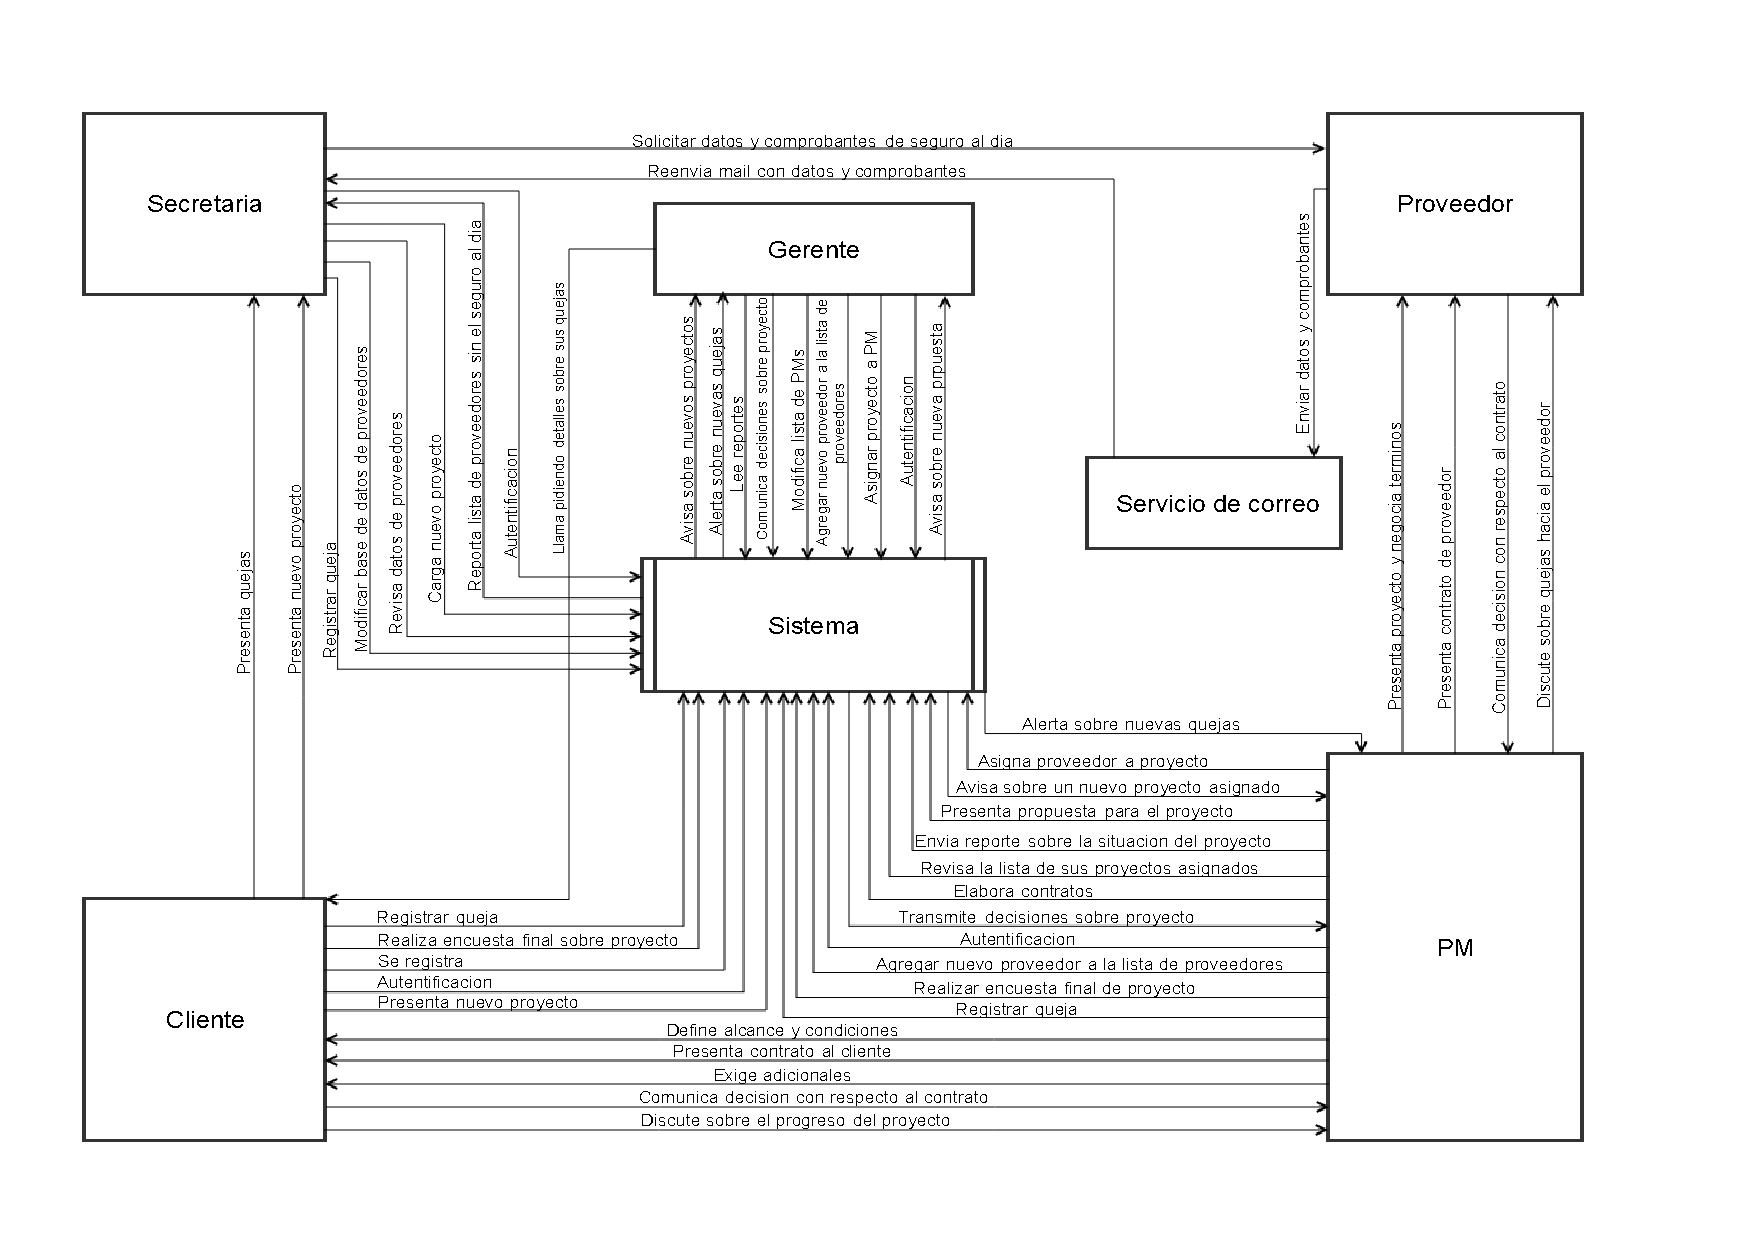
\includegraphics[width=\textheight/10*9,height=\textwidth,angle=90]{images/contexto.pdf}

\footnote{Notar que el cliente y el proveedor solo interactúan con los diferentes departamentos, no lo hacen directamente con el sistema.}

\section{Diagrama de Objetivos}

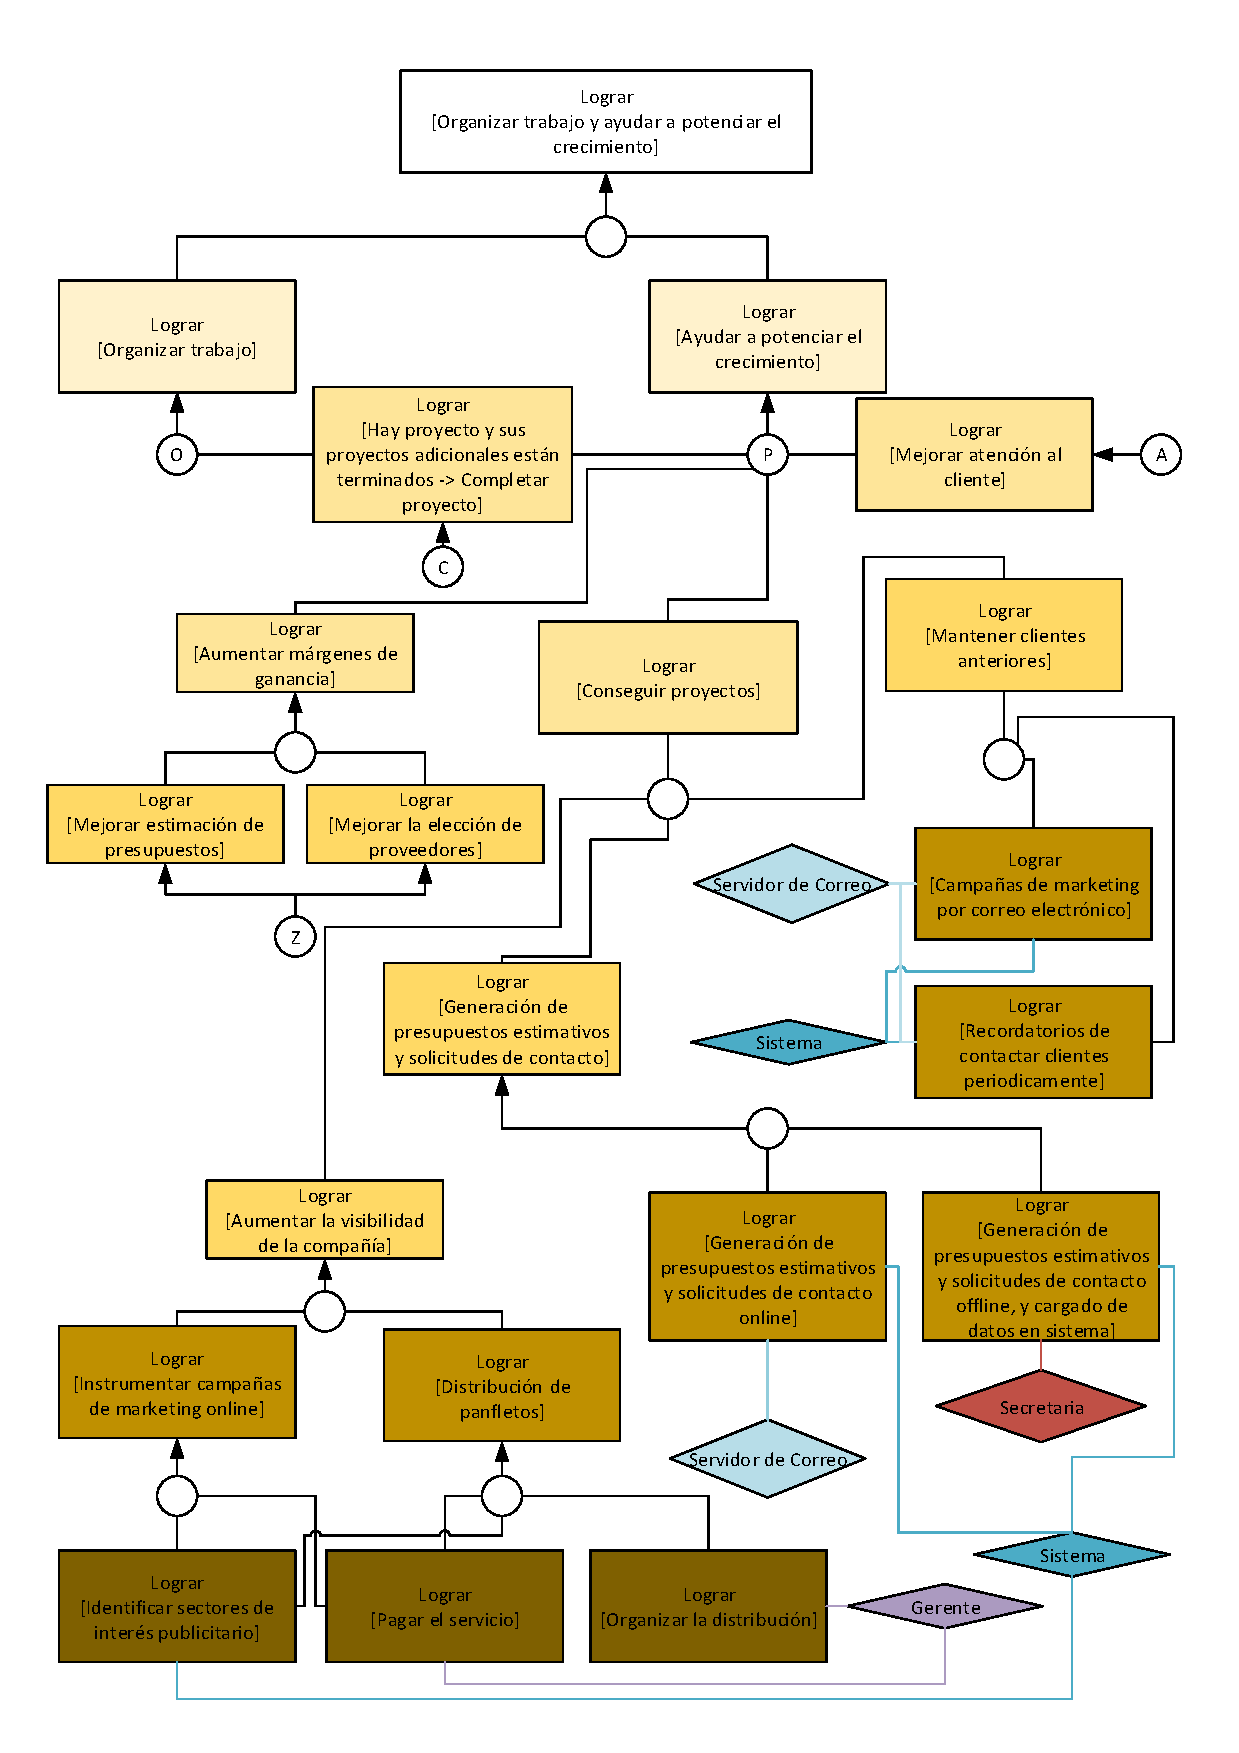
\includegraphics[width=\textwidth,height=\textheight,keepaspectratio,page=1]{images/objetivos.pdf}
\includegraphics[width=\textwidth,height=\textheight,keepaspectratio,page=2]{images/objetivos.pdf}
\includegraphics[width=\textwidth,height=\textheight,keepaspectratio,page=3]{images/objetivos.pdf}
\includegraphics[width=\textwidth,height=\textheight,keepaspectratio,page=4]{images/objetivos.pdf}
\includegraphics[width=\textwidth,height=\textheight,keepaspectratio,page=5]{images/objetivos.pdf}
\includegraphics[width=\textwidth,height=\textheight,keepaspectratio,page=6]{images/objetivos.pdf}
\includegraphics[width=\textwidth,height=\textheight,keepaspectratio,page=7]{images/objetivos.pdf}

\newcommand{\curef}[1]{\textbf{Caso de uso \ref{cu:#1}}}
\newcommand{\cutitle}[1]{\renewcommand{\givencutitle}{#1}}
\newcommand{\cuactors}[1]{\renewcommand{\givencuactors}{#1}}
\newcommand{\cupre}[1]{\renewcommand{\givencupre}{#1}}
\newcommand{\cupost}[1]{\renewcommand{\givencupost}{#1}}
\newcommand{\cucourse}[1]{\renewcommand{\givencucourse}{#1}}
\newcommand{\culabel}[1]{\renewcommand{\givenculabel}{#1}}
\newcommand{\cucaption}[1]{\renewcommand{\givencucaption}{#1}}
\newcommand{\givencutitle}{REQUIRED!}
\newcommand{\givencuactors}{REQUIRED!}
\newcommand{\givencupre}{-}
\newcommand{\givencupost}{-}
\newcommand{\givencucourse}{REQUIRED!}
\newcommand{\givenculabel}{REQUIRED!}
\newcommand{\givencucaption}{} % optional

\newenvironment{casodeuso}
{\begin{table}[H]}{%
\begin{tabular}{|p{0.5\linewidth} p{0.5\linewidth}|}\hline
\multicolumn{2}{|l|}{\textbf{Caso de Uso: \ref{cu:\givenculabel}) \givencutitle}} \\
\multicolumn{2}{|l|}{\textbf{Actor:} \givencuactors} \\
\multicolumn{2}{|l|}{\textbf{Pre:} \givencupre} \\
\multicolumn{2}{|l|}{\textbf{Post:} \givencupost} \\
\vspace{1px}\textbf{Curso Normal} & \vspace{1px}\textbf{Curso Alternativo} \\
\givencucourse
\hline
\end{tabular}
\caption{\givencutitle}
\label{cu:\givenculabel}
\end{table}}

\section{Casos de Uso}

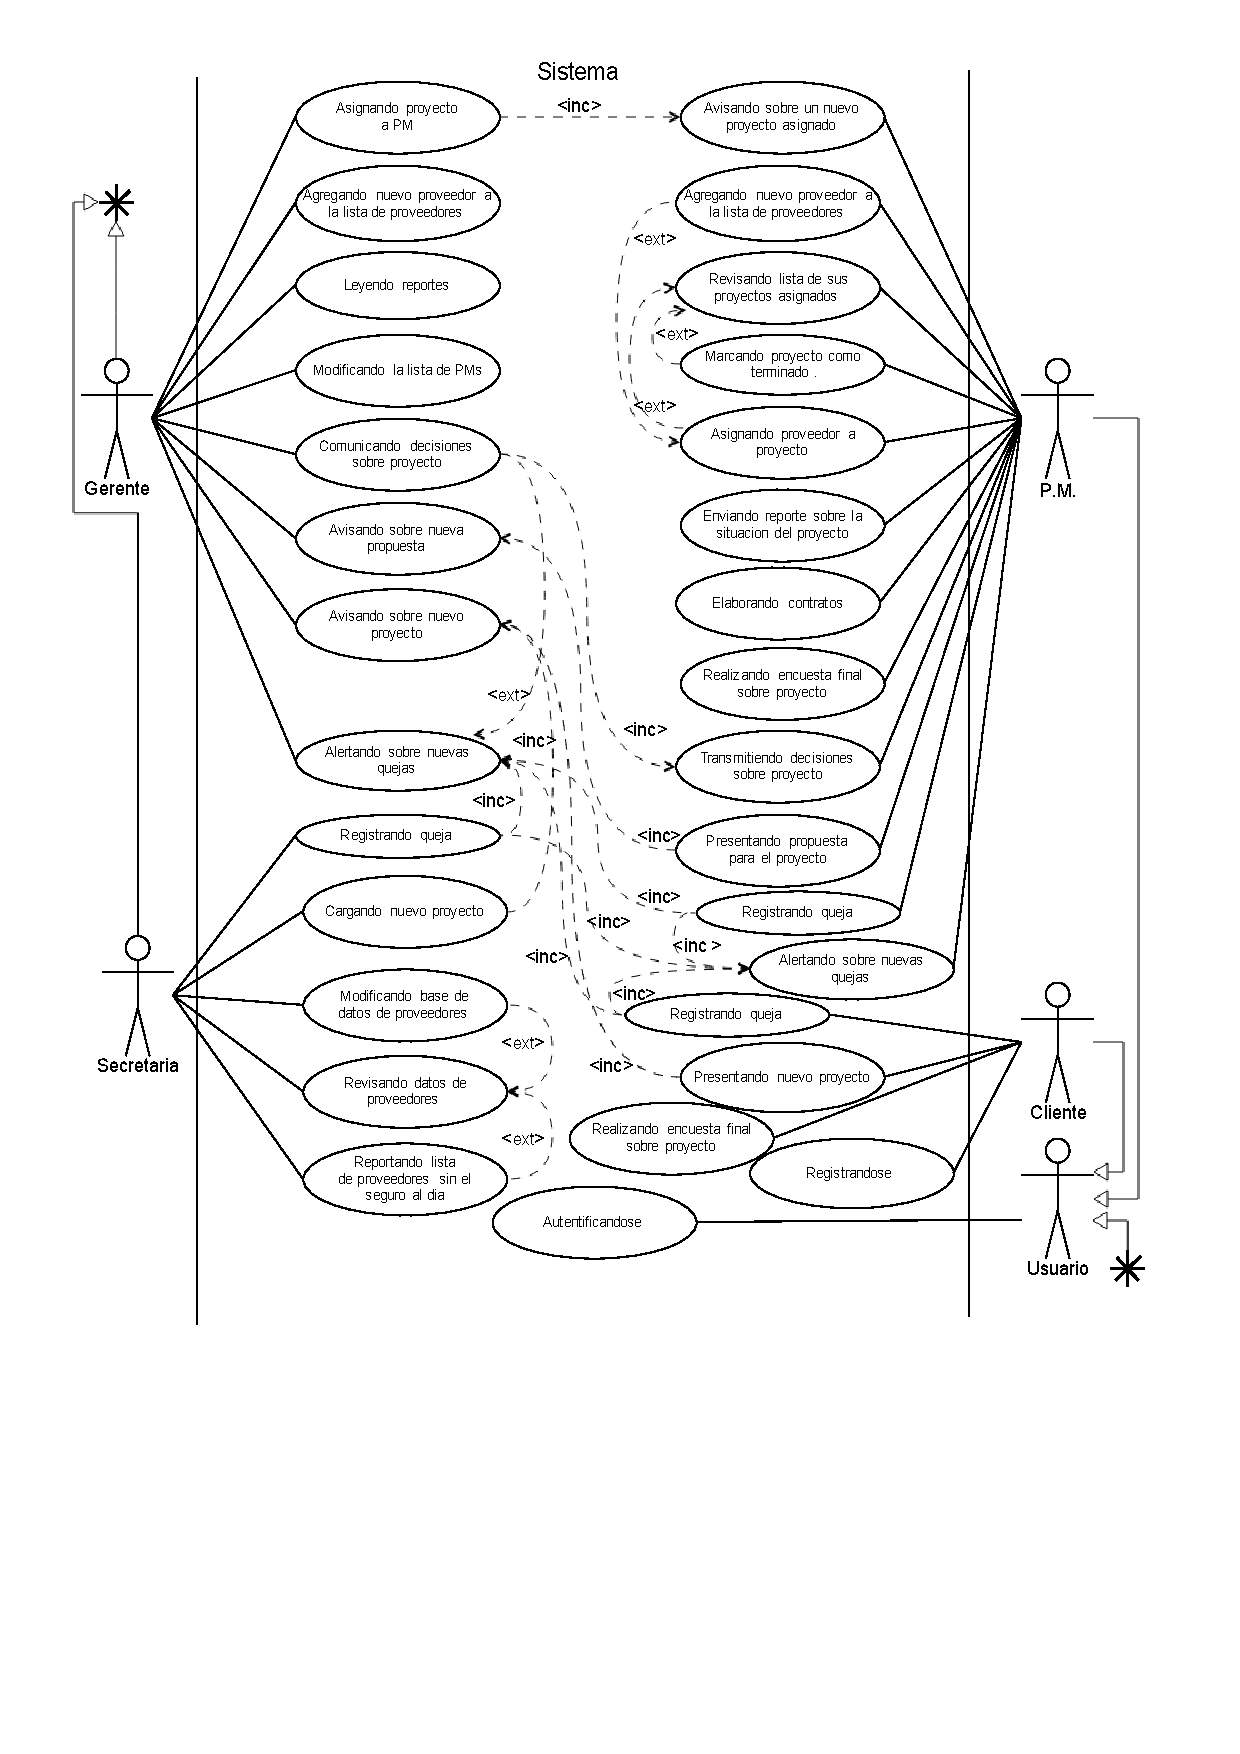
\includegraphics[width=\textwidth,height=\textheight,keepaspectratio,trim={0 1 cm 0 0},clip]{images/agentes.pdf}

\begin{casodeuso}
  \cutitle{Autentificandose}
  \cuactors{Usuario}
  \cupre{El cliente no esta ya autenticado}
  \cupost{El cliente esta autenticado}
  \cucourse{
    1. El Cliente ingresa sus datos & \\
    2. El Sistema verifica dichos datos & 2.1 Los datos son inválidos, se muestra un error por pantalla. Ir a 1 \\
    3. El Cliente es redirigido a la pantalla de inicio & \\
    4. Fin CU & \\
  }
  \culabel{autentificandose}
\end{casodeuso}


\begin{casodeuso}
  \cutitle{Registrándose}
  \cuactors{Cliente}
  \cupre{True}
  \cupost{El cliente se encuentra registrado en el sistema}
  \cucourse{
    1. El cliente ingresa usuario y contraseña & \\
    2. El sistema verifica que dicho usuario no este registrado & 2.1. Usuario ya registado, se muestra un error por pantalla. Ir a 1\\
    3. El cliente ingresa su nombre completo & \\
    4. El cliente ingresa su dirección de correo & \\
    5. El sistema verifica el correo & 5.1. Dirección de correo invalida, se muestra un error por pantalla. Ir a 4. \\
    6. El cliente ingresa sus dirección & \\
    7. El sistema verifica la validez de la dirección & 7.1. Dirección invalida, se muestra un error por pantalla. Ir a 6. \\
    8. El cliente ingresa su numero de teléfono & \\
    9. El sistema verifica dicho numero & 9.1. Numero invalido, se muestra un error por pantalla. Ir a 8.\\
    10. El sistema registra al nuevo usuario en el sistema & \\
    11. El sistema informa por pantalla que el registro fue exitoso & \\
    12. Fin CU & \\
    }
  \culabel{registrandose}
\end{casodeuso}

\begin{casodeuso}
  \cutitle{Realizando encuesta final sobre proyecto}
  \cuactors{Cliente}
  \cupre{El proyecto del cliente debe estar cargado en el sistema y estar en estado \textit{terminado}}
  \cupost{El cliente deja asentada su opinión acerca del proyecto}
  \cucourse{
    1. El sistema le presenta al cliente una serie de preguntas acerca del proyecto & \\
    2. El cliente contesta dichas preguntas & \\
    3. El sistema verifica que haya respondido todas las preguntas & 3.1. Quedaron preguntas sin contestar, se muestra un error por pantalla. Ir a 1. \\
    4. El sistema le pone una estampa de fecha y hora al formulario & \\
    5. El sistema archiva las respuestas del cliente & \\
    6. Fin CU & \\
    }
  \culabel{realizando-encuesta}
\end{casodeuso}

\begin{casodeuso}
  \cutitle{Realizando encuesta final sobre proyecto}
  \cuactors{PM}
  \cupre{El proyecto del cliente debe estar cargado en el sistema y haber concluido}
  \cupost{El PM deja asentada su opinión acerca del proyecto}
  \cucourse{
    1. El sistema le presenta al PM una serie de preguntas acerca del proyecto & \\
    2. El PM contesta dichas preguntas & \\
    3. El sistema verifica que haya respondido todas las preguntas & 3.1. Quedaron preguntas sin contestar, se muestra un error por pantalla. Ir a 1. \\
    4. El sistema le pone una estampa de fecha y hora al formulario & \\
    5. El sistema archiva las respuestas del PM & \\
    6. Fin CU & \\
    }
  \culabel{realizando-encuesta}
\end{casodeuso}

\begin{casodeuso}
  \cutitle{Presentando nuevo proyecto}
  \cuactors{Cliente}
  \cupre{El cliente debe estar autenticado en el sistema}
  \cupost{El proyecto del cliente queda registrado y en estado \textit{pendiente.} }
  \cucourse{
    1. El sistema le pide al cliente que describa el alcance del proyecto & \\
    2. El cliente escribe un breve texto explicando el proyecto que se desea realizar & \\
    3. El sistema archiva dicho texto & \\
    4. Incluye CU: Avisando sobre nuevo proyecto & \\
    5. Fin CU & \\
  }
  \culabel{presentando-nuevo-proyecto}
\end{casodeuso}

\begin{casodeuso}
  \cutitle{Presentando propuesta para el proyecto}
  \cuactors{PM}
  \cupre{El P.M. debe estar autenticado en el sistema}
  \cupost{La propuesta queda registrada en el sistema como \textit{pendiente.}}
  \cucourse{
    1. El sistema le pide al P.M. que describa el alcance de la propuesta & \\
    2. El P.M. ingresa un texto explicando dicha propuesta & \\
    3. El sistema archiva el texto & \\
    4. El sistema marca el estado de la propuesta como \textit{pendiente.} & \\
    5. Incluye CU: Avisando sobre nueva propuesta & \\
    6. Fin CU & \\
    }
    \culabel{presentando-prop}
\end{casodeuso}

\begin{casodeuso}
  \cutitle{Transmitiendo decisiones sobre proyecto}
  \cuactors{PM}
  \cupre{El PM debe tener un proyecto asignado}
  \cupost{El PM es notificado de las decisiones del gerente}
  \cucourse{
    1. Si el PM se encuentra autenticado, el sistema interrumpe brevemente al PM para mostrar un informe con nuevas decisiones que el gerente tomo acerca del proyecto & 1.1. Si el PM no se encuentra autentificado, se lo notifica en el portal principal al momento de su próxima autentificación \\
    2. El P.M. acepta la notificación y continua con sus actividades en el sistema & \\
    3. Fin CU & \\
    }
  \culabel{transmitiendo}
\end{casodeuso}

\begin{casodeuso}
  \cutitle{Elaborando contratos}
  \cuactors{PM}
  \cupre{El PM debe estar autenticado en el sistema y tener al menos un proyecto a su cargo sin contrato}
  \cupost{El contrato queda elaborado}
  \cucourse{
    1. El sistema le presenta al P.M. una selección de templates de contratos de cliente y proveedor para elegir & 1.1. El proyecto no tiene proveedor asignado, se muestra un error por pantalla. Fin CU. \\
    2. El P.M. selección los templates de contrato según su criterio & \\
    3. El sistema genera los nuevos contratos en base al template & \\
    4. El sistema le pide al P.M. que indique la fecha de inicio de la obra & \\
    5. El P.M. ingresa la fecha & \\
    6. El sistema le pide al P.M. que indique la fecha de fin de la obra & \\
    7. El P.M. ingresa la fecha & \\
    8. El sistema le pide al P.M. que cambie los términos de los contratos si lo desea & \\
    9. El P.M. cambia los términos de los contratos según sea necesario & \\
    10. El sistema le pide que ingrese el monto total por la obra & \\
    11. El P.M. ingresa el monto & \\
    12. El sistema marca los contratos como no firmados & \\
    13. El sistema archiva los contratos elaborados & \\
    14. Fin CU & \\
    }
    \culabel{elaborando-contratos}
\end{casodeuso}

\begin{casodeuso}
  \cutitle{Enviando reporte sobre la situación del proyecto}
  \cuactors{PM}
  \cupre{El PM debe estar autenticado en el sistema y tener al menos un proyecto a su cargo}
  \cupost{El reporte queda archivado en el sistema}
  \cucourse{
    1. El sistema le pide al PM que ingrese un texto describiendo el estado actual del proyecto & \\
    2. El PM escribe el texto describiendo las ultimas novedades & \\
    3. El sistema le coloca una estampa de fecha y hora al formulario & \\
    4. El sistema archiva el reporte & \\
    5. Fin CU & \\
    }
    \culabel{enviando-reporte}
\end{casodeuso}

\begin{casodeuso}
  \cutitle{Asignando proveedor a proyecto}
  \cuactors{PM}
  \cupre{El PM debe estar autenticado en el sistema y tener al menos un proyecto a su cargo}
  \cupost{El proyecto tiene un proveedor asignado}
  \cucourse{
    1. El sistema le proporciona al PM una lista de posibles proveedores para elegir & 1.1. El PM no tiene proyectos sin proveedor asignado, se muestra un error en pantalla. Fin CU. \\
    2. El P.M. realiza la decisión sobre cual elegir según su discreción & 2.1. No hay proveedores disponibles y/o acordes al rubro del proyecto, se extiende al CU: Agregando nuevo proveedor a la lista de proveedores. Ir a 2.\\
    3. El sistema guarda la decisión del PM & \\
    4. Fin CU & \\
    }
    \culabel{asignando-proveedor}
\end{casodeuso}

\begin{casodeuso}
  \cutitle{Revisando la lista de proyectos asignados}
  \cuactors{PM}
  \cupre{El PM debe estar autenticado en el sistema}
  \cupost{Los proyectos aprobados cuentan con un proveedor asignado}
  \cucourse{
    1. El sistema le presenta una lista de los proyectos asignados al PM & \\
    2. El PM revisa dicha lista verificando el estado de los proyectos & 2.1. El PM no tiene proyectos asignados, se muestra un error en pantalla. Fin CU. & \\
    3. El PM revisa que los proyectos con propuesta activa tengan sus proveedores asignados & 3.1. Existen proyectos con propuestas activas que no tienen ningun proveedor asignado, se extiende al CU: Asignando proveedor a proyecto & \\
    4. El PM revisa que los proyectos que hayan concluido figuren como \textit{terminados} & 4.1. Se encuentra con que hay proyectos que concluyeron pero no figuran como \textit{terminados}, se extiende al CU: Marcando proyecto como terminado.
    5. Fin CU & \\
    }
    \culabel{revisando-lista-proyectos}
\end{casodeuso}

\begin{casodeuso}
  \cutitle{Agregando nuevo proveedor a la lista de proveedores}
  \cuactors{PM}
  \cupre{El PM debe estar autenticado}
  \cupost{Un nuevo proveedor es agregado a la lista de proveedores}
  \cucourse{
    1. El PM ingresa la direccion del proveedor & \\
    2. El sistema verifica la direccion &  2.1. Direccion invalida, se muestra un error por pantalla. Ir a 1. \\
    3. El PM ingresa el telefono del proveedor & \\
    4. El sistema veriica dicho numero & 4.1. Numero invalido, se muestra un error por pantalla. Ir a 3. \\
    5. El sistema marca al proveedor como ingresado por PM & \\
    6. El sistema coloca una estampa de fecha y hora al formulario & \\
    7. Fin CU & \\
    }
\end{casodeuso}

\begin{casodeuso}
  \cutitle{Avisando sobre un nuevo proyecto asignado}
  \cuactors{PM}
  \cupre{True}
  \cupost{El PM es notificado de que se le ha asignado un nuevo proyecto}
  \cucourse{
    1. Si el PM se encuentra autenticado, el sistema interrumpe brevemente al PM para indicarle que le fue asignado un nuevo proyecto & 1.1. Si el PM no se encuentra autentificado, se lo notifica en el portal principal al momento de su próxima autentificación & \\
    2. El P.M. acepta la notificación y continua con sus actividades en el sistema & \\
    3. Fin CU & \\
    }
    \culabel{avisando-nuevo-proyecto-asignado}
\end{casodeuso}

\begin{casodeuso}
  \cutitle{Asignando proyecto a PM}
  \cuactors{Gerente}
  \cupre{El Gerente debe estar autenticado y debe haber al menos un proyecto en sistema sin PM}
  \cupost{El proyecto pasa a estar en estado \textit{asignado}}
  \cucourse{
    1. El sistema le ofrece una lista de PMs al gerente para que elija & No hay gerentes registrados en sistema. Ir a Fin CU & \\
    2. El gerente elije un PM para el proyecto según su discreción & \\
    3. Incluyendo CU: Avisando sobre nuevo proyecto asignado & \\
    4. Fin CU & \\
    }
    \culabel{asignando-proyecto-pm}
\end{casodeuso}

\begin{casodeuso}
  \cutitle{Agregando nuevo proveedor a la lista de proveedores}
  \cuactors{Gerente}
  \cupre{El gerente debe estar autenticado}
  \cupost{Un nuevo proveedor es agregado a la lista de proveedores}
  \cucourse{
    1. El gerente ingresa la direccion del proveedor & \\
    2. El sistema verifica la direccion &  2.1. Direccion invalida, se muestra un error por pantalla. Ir a 1. & \\
    3. El gerente ingresa el telefono del proveedor & \\
    4. El sistema veriica dicho numero & 4.1. Numero invalido, se muestra un error por pantalla. Ir a 3. \\
    5. El sistema marca al proveedor como ingresado por gerente & \\
    6. El sistema coloca una estampa de fecha y hora al formulario & \\
    7. Fin CU & \\
    }
\end{casodeuso}

\begin{casodeuso}
  \cutitle{Leyendo reportes}
  \cuactors{Gerente}
  \cupre{El gerente debe estar autenticado}
  \cupost{El gerente lee los reportes de los diferentes proyectos}
  \cucourse{
    1. El sistema le provee al gerente la lista de proyectos disponibles & 1.1. No hay reportes en el sistema para leer, se muestra un error en pantalla. Fin CU.& \\
    2. El gerente elige el proyecto sobre el cual desea informarse & \\
    3. El sistema le presenta en pantalla los reportes disponibles al gerente & \\
    4. El gerente elige el reporte que desea & \\
    5. El sistema le provee el reporte al gerente & \\
    6. Fin CU & \\
    }
    \culabel{leyendo-reportes}
\end{casodeuso}

\begin{casodeuso}
  \cutitle{Modificando lista de PMs}
  \cuactors{Gerente}
  \cupre{El gerente debe estar autenticado}
  \cupost{El gerente modifica la lista de PMs}
  \cucourse{
   1. El sistema le presenta al gerente la lista de PMs actuales & \\
   2. El gerente agrega o remueve PMs según su discreción & \\
   3. El sistema archiva la lista modificada de PMs & \\
   4. Fin CU & \\
   }
   \culabel{modificando-lista}
\end{casodeuso}

\begin{casodeuso}
  \cutitle{Comunicando decisiones sobre proyecto}
  \cuactors{Gerente}
  \cupre{El gerente debe estar autenticado y el proyecto debe tener un PM asignado}
  \cupost{El gerente expresa su opinion de la propuesta y se notifica al PM}
  \cucourse{
    1. El sistema le muestra al gerente las propuestas cargadas por el PM actual & \\
    2. El gerente pone notas del alcance actual segun su discrecion & \\
    3. El gerente en caso de haber tomado una decision final, aprueba o rechaza la propuesta & \\
    4. En caso de haberse marcado un cambio de estado, el sistema actualiza el estado de la propuesta, pasando a estar activa en caso de que haya sido aprobada, y en caso de haberla, desactivando la propuesta activa precedente & \\
    4. Incluye CU: Transmitiendo decisiones sobre proyecto & \\
    5. Fin CU & \\
    }
    \culabel{comunicando}
\end{casodeuso}

\begin{casodeuso}
  \cutitle{Avisando sobre un nuevo proyecto asignado}
  \cuactors{Gerente}
  \cupre{True}
  \cupost{El gerente es notificado del nuevo proyecto}
  \cucourse{
    1. Si el gerente se encuentra autenticado, el sistema interrumpe brevemente al gerente para indicarle que le fue asignado un nuevo proyecto & 1.1. Si el gerente no se encuentra autenticado, se lo notifica en el portal principal al momento de su próxima autentificacion & \\
    2. El gerente acepta la notificación y continua con sus actividades en el sistema & \\
    3. Fin CU & \\
    }
    \culabel{avisando-proyecto-asignado}
\end{casodeuso}

\begin{casodeuso}
  \cutitle{Cargando nuevo proyecto}
  \cuactors{Secretaria}
  \cupre{La secretria debe estar autenticada}
  \cupost{El proyecto queda registrado en el sistema en estado \textit{pendiente.}}
  \cucourse{
    1. El sistema le pide a la secretaria que describa el alcance del proyecto & \\
    2. La secretaria escribe un breve texto explicando el proyecto que se desea realizar & \\
    3. El sistema archiva dicho texto & \\
    4. Incluye CU: Avisando sobre nuevo proyecto & \\
    5. Fin CU & \\
    }
  \culabel{presentando-proyecto-secretaria}
\end{casodeuso}

\begin{casodeuso}
  \cutitle{Modificando base de datos de proveedores}
  \cuactors{Secretaria}
  \cupre{La secretaria debe esta autenticada}
  \cupost{La base de datos de proveedores queda modificada}
  \cucourse{
    1. El sistema le provee una lista de proveedores & \\
    2. La secretaria agrega o borra proveedores segun su discrecion \\
    3. El sistema provee los datos del proveedor que se desea modificar \\
    4. La secretaria modifica los datos \\
    5. El sistema archiva los cambios \\
    6. Fin CU \\
    }
  \culabel{modificando-base}
\end{casodeuso}

\begin{casodeuso}
  \cutitle{Revisando datos de proveedores}
  \cuactors{Secretaria}
  \cupre{La secretaria debe estar autenticada}
  \cupost{Se proveen los datos del proveedor}
  \cucourse{
    1. El sistema le provee una lista de proveedores & \\
    2. La secretaria elige el proveedor que desea consultar & 2.1. El proveedor no se encuentra en sistema, se imprime un error por pantalla. Fin CU. & \\
    3. El sistema le provee los datos del proveedor & \\
    4. En caso de que necesite asegurarse que algun proveedor ademas tenga el seguro al dia, extiende CU: Reportando lista de proveedores sin el seguro al dia. & \\
    5. En caso de que se encuentre con que hay datos desactualizados con respecto a la ultima documentacion enviada por el proveedor, extiende a CU: Modificando base de datos de proveedores. Ir a 2. & \\
    6. Fin CU & \\
    }
  \culabel{revisando-proveedor}
  
\end{casodeuso}

\begin{casodeuso}
  \cutitle{Reportando lista de proveedores sin el seguro al dia}
  \cuactors{Secretaria}
  \cupre{La secretaria debe estar autenticada}
  \cupost{El sistema provee una lista de proveedores sin seguro al dia}
  \cucourse{
    1. El sistema reporta una lista con todos proveedores que no tengan el seguro al dia.& \\
    2. Fin CU & \\}
  \culabel{sin-seguro}
\end{casodeuso}

\begin{casodeuso}
  \cutitle{Marcando proyecto como terminado}
  \cuactors{PM}
  \cupre{El PM debe estar autenticado}
  \cupost{El proyecto seleccionado pasa a estar en estado \textit{terminado.}}
  \cucourse{
    1. El PM selecciona un proyecto de su lista de proyectos asignados & 1.1. El PM no tiene proyectos asignado. Ir a Fin CU & \\
    2. El PM tilda el proyecto seleccionado como Terminado & \\
    3. El Sistema registra el cambio. & 3.1. El Sistema rechaza el cambio de estado, e indica que no hay una propuesta activa para el proyecto. & \\
    4. Fin CU & \\}
  \culabel{sin-seguro}
\end{casodeuso}

\begin{casodeuso}
  \cutitle{Registrando queja}
  \cuactors{PM}
  \cupre{El PM debe estar autenticado}
  \cupost{La queja queda registrada y asociada a los correspondientes agentes}
  \cucourse{
    1. El PM selecciona el proyecto de su lista de proyectos asignados para el cual el cliente tiene la queja & 1.1. El proyecto del cual habla la queja no esta asignado al PM. Ir a Fin CU. & \\
    2. El PM registra la queja asociandola ademas con los agentes que estan involucrados en el reclamo. & \\
    3. El Sistema archiva la queja. & \\
    4. El sistema oportunamente alerta al Gerente sobre la nueva queja. Usa CU: Alertando sobre nuevas quejas. & \\
    5. Fin CU & \\}
  \culabel{sin-seguro}
\end{casodeuso}

\begin{casodeuso}
  \cutitle{Registrando queja}
  \cuactors{Cliente}
  \cupre{El Cliente debe estar autenticado}
  \cupost{La queja queda registrada y asociada a los correspondientes agentes}
  \cucourse{
    1. El Cliente selecciona el proyecto de su lista de proyectos presentados para el cual el cliente tiene la queja & \\
    2. El Cliente registra la queja asociandola ademas con los agentes que estan involucrados en el reclamo. & \\
    3. El Sistema archiva la queja. & \\
    4. El sistema oportunamente alerta al Gerente sobre la nueva queja. Usa CU: Alertando sobre nuevas quejas. & \\
    5. El sistema alerta sobre una nueva queja al PM asociado al proyecto del cual se refiere la queja. Usa CU: Alertando sobre nuevas quejas. & \\
    6. Fin CU & \\}
  \culabel{sin-seguro}
\end{casodeuso}

\begin{casodeuso}
  \cutitle{Registrando queja}
  \cuactors{Secretaria}
  \cupre{La Secretaria debe estar autenticada}
  \cupost{La queja queda registrada y asociada a los correspondientes agentes}
  \cucourse{
    1. La secretaria selecciona el proyecto pertinente de la lista de proyectos presentados por el cliente que tiene la queja & \\
    2. La secretaria registra la queja pasada telefonicamente por el Cliente, asociandola ademas con los agentes que estan involucrados en el reclamo.
    3. El Sistema archiva la queja. & \\
    4. El sistema oportunamente alerta al Gerente sobre la nueva queja. Usa CU: Alertando sobre nuevas quejas. & \\
    5. El sistema alerta sobre una nueva queja al PM asociado al proyecto del cual se refiere la queja. Usa CU: Alertando sobre nuevas quejas. & \\
    6. Fin CU & \\}
  \culabel{sin-seguro}
\end{casodeuso}

\begin{casodeuso}
  \cutitle{Alertando queja}
  \cuactors{PM}
  \cupre{El PM debe estar autenticado}
  \cupost{El PM queda informado acerca de las quejas asociadas a sus proyectos}
  \cucourse{
    1. El sistema ni bien el PM se autentica le presenta a un costado de la pantalla en una lista de quejas, y en rojo, las nuevas quejas relacionadas con sus proyectos asignados & \\
    2. El PM las revisa, y las marca como leidas.
    3. El Sistema registra las alertas confirmadas. & \\
    4. Fin CU & \\}
  \culabel{sin-seguro}
\end{casodeuso}

\begin{casodeuso}
  \cutitle{Alertando queja}
  \cuactors{Gerente}
  \cupre{El gerente debe estar autenticado}
  \cupost{El gerente queda informado acerca de las quejas asociadas a sus proyectos}
  \cucourse{
    1. El sistema le presenta oportunamente segun la configuracion propia de la cuenta con la que el gerente se autentico; a un costado de la pantalla, una lista de nuevas quejas clasificadas en leidas y no leidas.  & \\
    2. El gerente las revisa, y las marca como leidas. & \\
    3. El Sistema registra las alertas confirmadas. & \\
    4. En caso de que el gerente considere necesario interferir, se extiende a CU: Comunicando decisiones sobre proyecto & \\
    5. Fin CU & \\}
  \culabel{sin-seguro}
\end{casodeuso}

\pagebreak

\section{Modelo Conceptual}

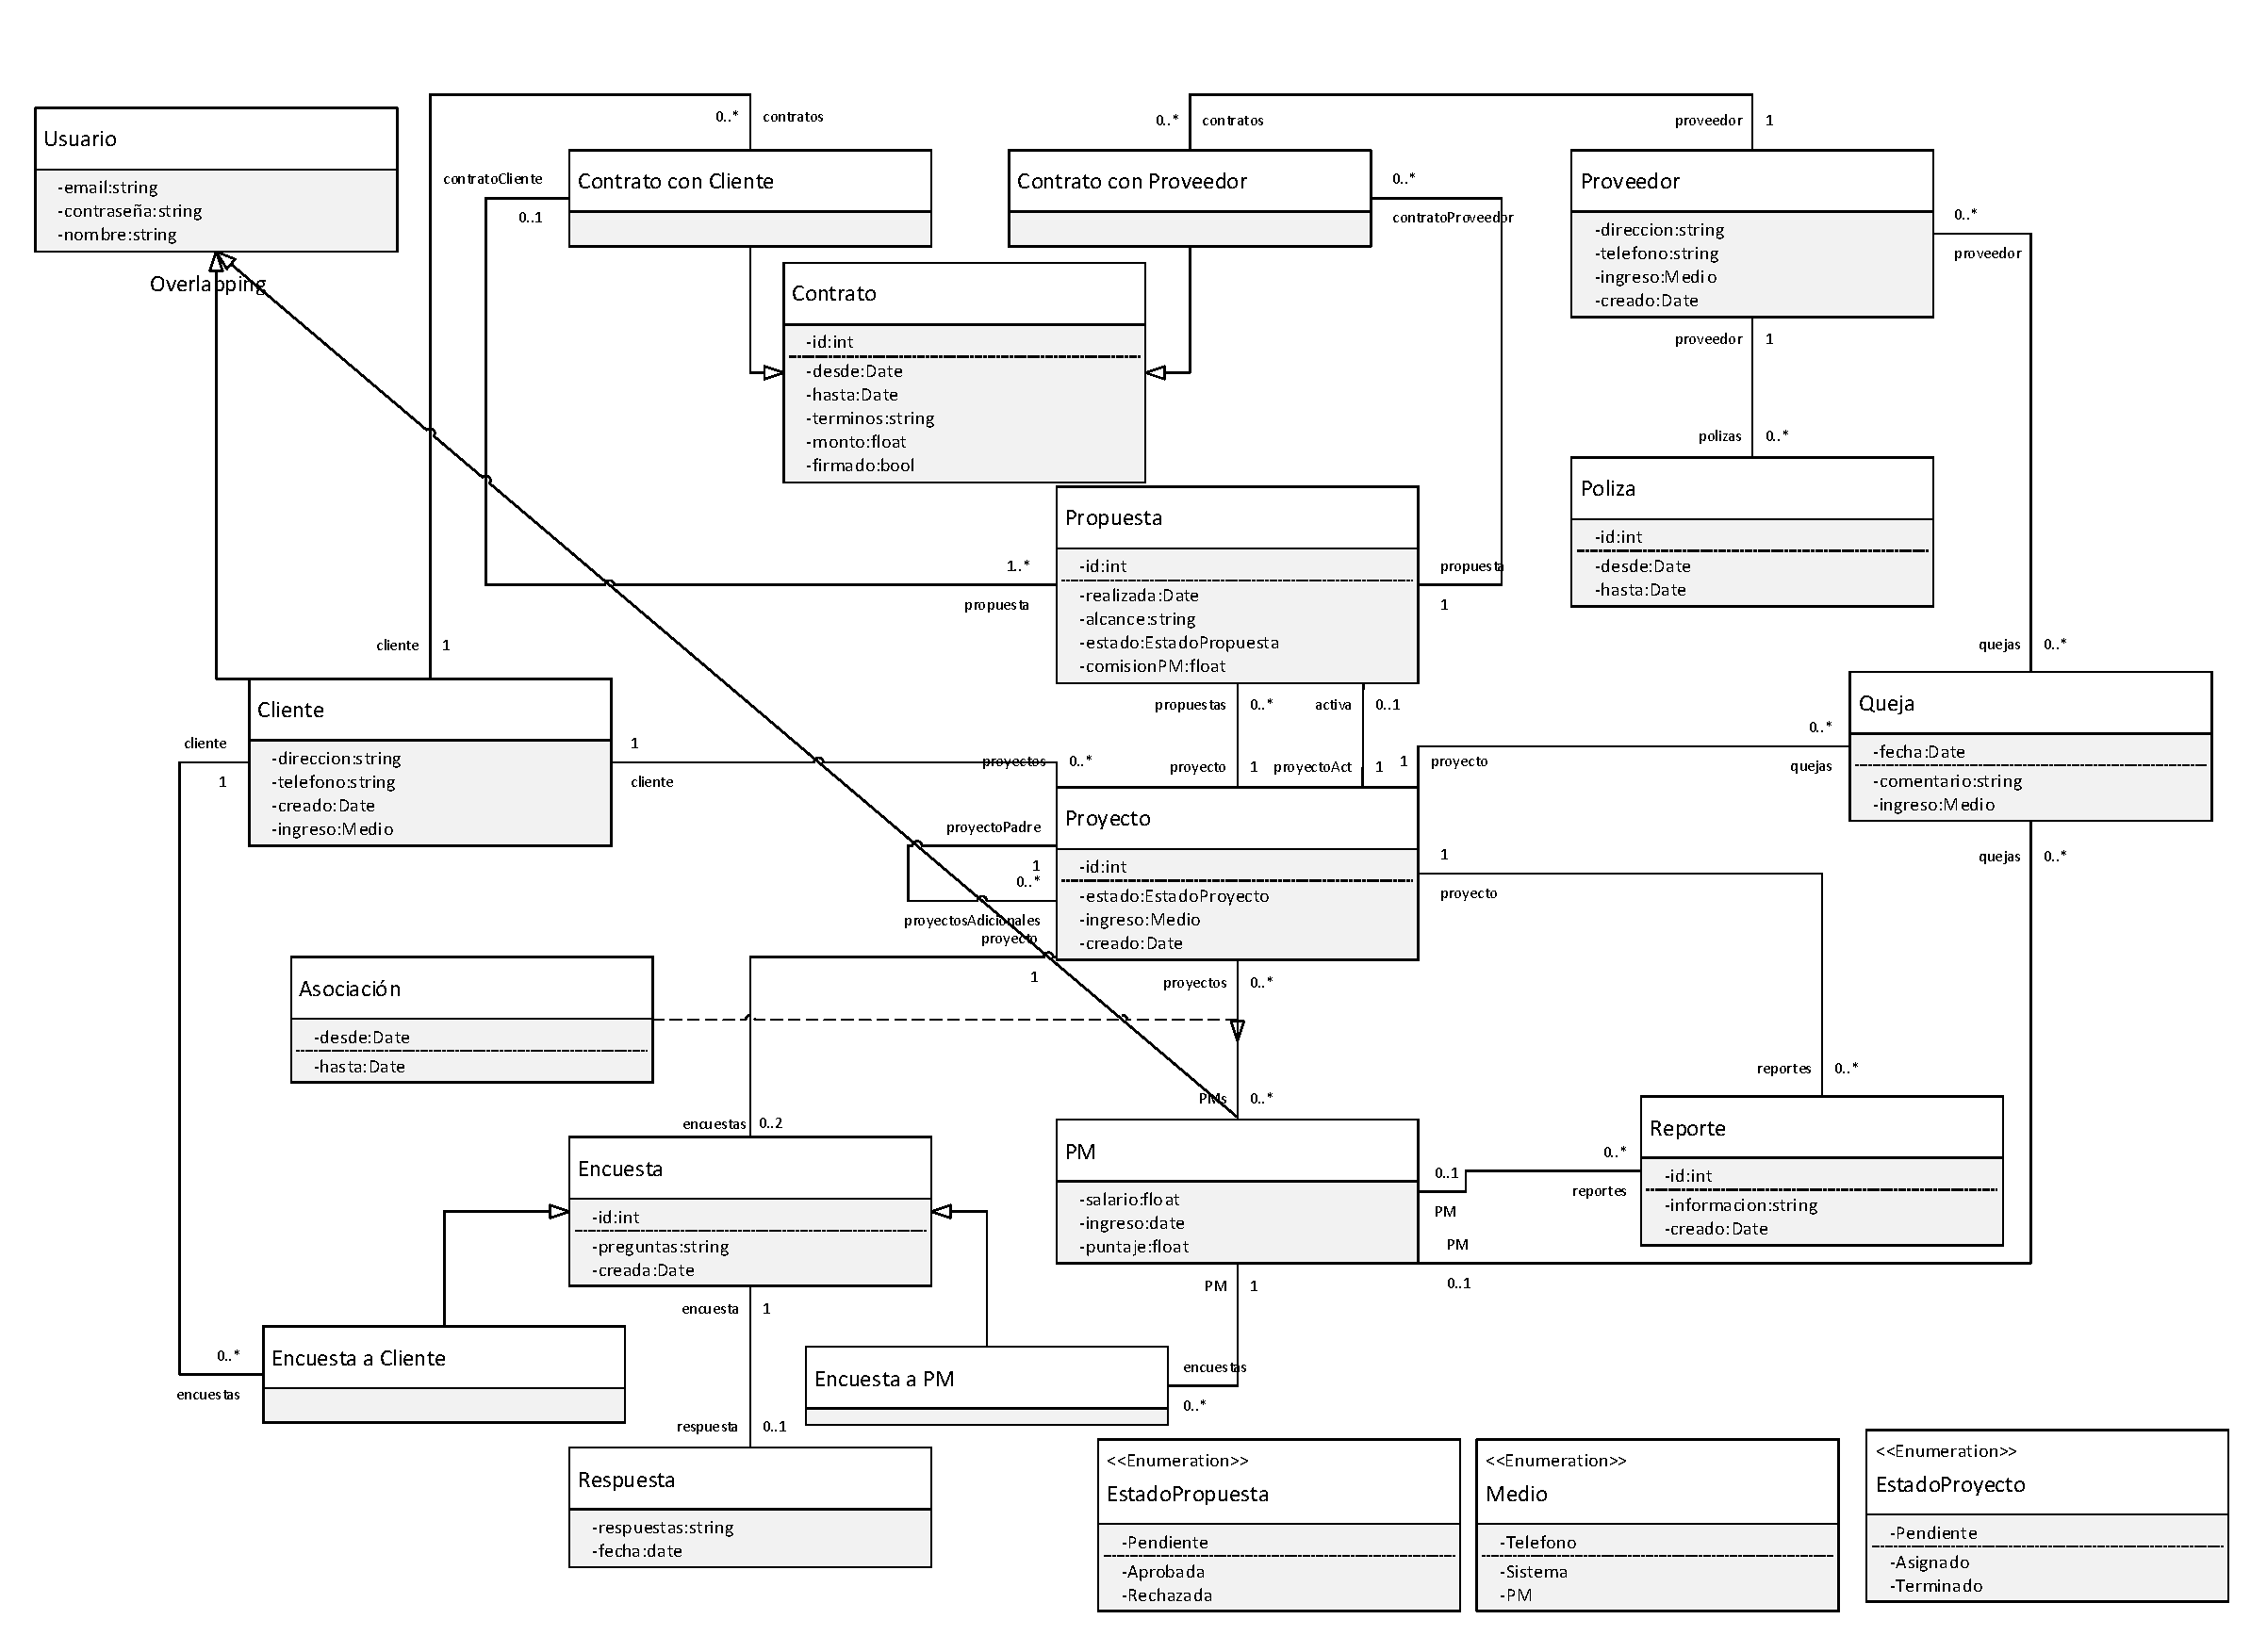
\includegraphics[height=\textwidth,angle=-270]{images/conceptual.pdf}

\pagebreak

Dado que la sintaxis de los diagramas de clases es limitada, agregamos las siguientes restricciones al mismo utilizando OCL (Object Constraint Language):

\begin{enumerate}
    \item Todo usuario tiene un email único y una contraseña no vacía.
    \item Todo PM tiene un salario mayor a 0.
    \item El puntaje de un PM es mayor o igual a 0.
    \item Todas las asociaciones de un PM tienen un desde mayor o igual que la fecha de ingreso del PM.
    
    \item Toda póliza tiene un ID único.
    \item La fecha de comienzo de una póliza debe ser menor o igual a la fecha de fin de la misma.
    \item La fecha de finalización de una póliza debe ser mayor o igual a la fecha de creación del proveedor al que está asociada.
    
    \item Todo contrato tiene un ID único.
    \item La fecha de comienzo de un contrato es menor a la de finalización.
    \item Los términos de un contrato son no vacíos.
    \item El monto de un contrato siempre es positivo.
    \item Un contrato con un proveedor debe tener pólizas de seguro asociadas para cada uno de los días cubiertos en el período.
    \item La fecha de comienzo de un contrato con un proveedor es menor o igual a la fecha de creación del proveedor.
    \item La fecha de comienzo de un contrato con un cliente es menor o igual a la fecha de creación del cliente.
    
    \item Toda propuesta tiene un ID único.
    \item Toda propuesta creada después del primer contrato firmado con el cliente tiene el mismo contrato con el cliente (es decir, el contrato firmado con el cliente no cambia con la propuesta).
    \item Toda propuesta activa tiene que tener su estado como aprobada.
    \item Los contratos solo pueden esta firmados si la propuesta asociada fue aprobada.
   % \item El proyecto debe ser igual al proyecto Act, en el caso en que este último exista.
    \item Para una propuesta, el cliente con el que se firma el contrato es exactamente el mismo que comenzó el proyecto al que pertenece la propuesta.
    \item La fecha de realización de una propuesta es menor o igual a la fecha de comienzo de un contrato
    \item El alcance de una propuesta es no vacío.
    \item La fecha de comienzo del contrato con el cliente debe ser menor o igual a la fecha de comienzo de todos los contratos con los proveedores, y la fecha de finalización del contrato activo con el cliente debe ser mayor o igual a la fecha de finalización de todos los contratos con los proveedores.
    \item El cliente asociado a una propuesta es el mismo que el que está asociado al proyecto con el que está asociada la propuesta.
    \item La comisión del PM debe ser mayor a 0
    
    \item Todo proyecto tiene un ID único.
    \item Todo proyecto adicional asociado tiene el mismo cliente que el proyecto padre, y una fecha de creación mayor o igual a la del proyecto padre.
    \item Si un proyecto esta en estado terminado, entonces tiene una propuesta activa.
    \item Los intervalos de asociación con un PM cubren completamente el intervalo de fechas desde el comienzo al fin del proyecto, y siempre hay un único PM para cada día.
    
    %% TODO: escribir bien
    \item Un proyecto está en estado terminado implica que todos sus proyectos hijos están terminados.
    \item Todo reporte tiene un ID único.
    \item La fecha de creación de un reporte es mayor o igual a la fecha de creación del proyecto al que está asociado.
    \item El string de información en un reporte es no vacío.
    \item El PM asociado a un reporte es el que estaba vigente en el momento en que se creó el reporte.
    \item La fecha de creación de una queja es mayor o igual a la fecha de creación del proyecto al que está asociada.
    \item El comentario de una queja es no vacío.
    \item La queja está asociada a por lo menos un proveedor o un PM (puede también estar asociada a ambos)
    \item El proveedor asociado a una queja tiene un contrato con el proyecto que abarca a la fecha de creación.
    \item El PM asociado a una queja estuvo asignado al proyecto en un intervalo que abarca a la fecha de creación de la queja.
    \item Toda encuesta tiene un ID único
    \item Toda encuesta a cliente tiene como cliente al mismo que está asociado al proyecto.
    \item Toda encuesta a PM tiene como PM al mismo que está asociado al proyecto.
    \item El string de preguntas es no vacío.
    \item Una respuesta es igual a otra si y sólo sí su encuesta es igual a la de la otra.
    \item La fecha de una respuesta es mayor o igual a la de su entrevista asociada.
    \item El string de respuestas es no vacío.
\end{enumerate}

\pagebreak

\section{Object Constraint Language Restrictions}

Algunas de estas restricciones se expresan en OCL de la siguiente manera:

\subsection*{Todo usuario tiene un email único y una contraseña no vacía.}

\begin{ocl}{}
Context: Usuario

inv:
Usuario.allInstances(u1,u2|u1 != u2 implies u1.email != u2.email) and self.contrasena.length() > 0
\end{ocl}

\subsection*{La fecha de finalización de una póliza debe ser mayor o igual a la fecha de creación del proveedor al que está asociada.}

\begin{ocl}{}
Context: Poliza

inv:
self.hasta >= self.proveedor.creado

\end{ocl}

\subsection*{Un contrato con un proveedor debe tener pólizas de seguro asociadas para cada uno de los días cubiertos en el período.}

\begin{ocl}{}
Context: Contrato con Proveedor

inv:
Date.forAll(d|d >= self.desde and d <= self.hasta implies self.proveedor.polizas.select(p|p.desde >= d and p.hasta <= d).count() > 0)

\end{ocl}

\subsection*{La fecha de comienzo del contrato con el cliente debe ser menor o igual a la fecha de comienzo de todos los contratos con los proveedores, y la fecha de finalización del contrato activo con el cliente debe ser mayor o igual a la fecha de finalización de todos los contratos con los proveedores.}

\begin{ocl}{}
Context: Propuesta

inv:
self.contratoProveedor.forAll(cp|self.contratoCliente.desde <= cp.desde)

\end{ocl}

\subsection*{Un proyecto está en estado terminado implica que todos sus proyectos hijos están terminados.}

\begin{ocl}{}
Context: Proyecto

inv:
self.estado = 'Terminado' implies self.proyectosAdicionales.forAll(p|p.estado = 'Terminado')

\end{ocl}

\subsection*{Toda propuesta activa tiene que tener su estado como aprobada.}

\begin{ocl}{}
Context: Proyecto

inv:
self.activa.estado = 'Aprobada'

\end{ocl}

\subsection*{Si un proyecto esta en estado terminado, entonces tiene una propuesta activa.}

\begin{ocl}{}
Context: Proyecto

inv:
self.estado = 'Terminado' implies self.activa->select(p|p.estado = 'Activa')->size() > 0

\end{ocl}

\pagebreak

\section{Diagramas de Actividad}

En los siguientes diagramas veremos como ciertos procesos, los que consideramos mas importantes, se llevan a cabo, viendo como interactúa cada agente que participa del mismo.


\makebox[\textwidth][c]{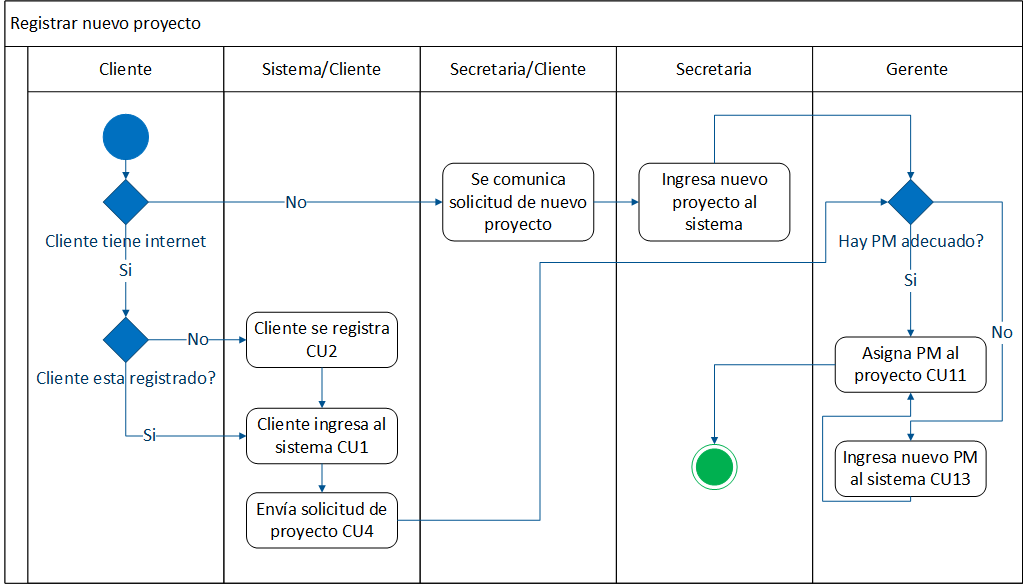
\includegraphics[width=1.15\textwidth]{images/RegProy.png}}
\makebox[\textwidth][c]{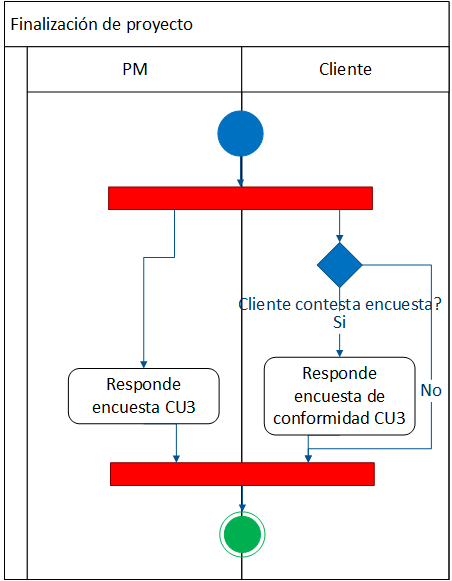
\includegraphics[width=0.55\textwidth]{images/FinProy.png}}
\makebox[\textwidth][c]{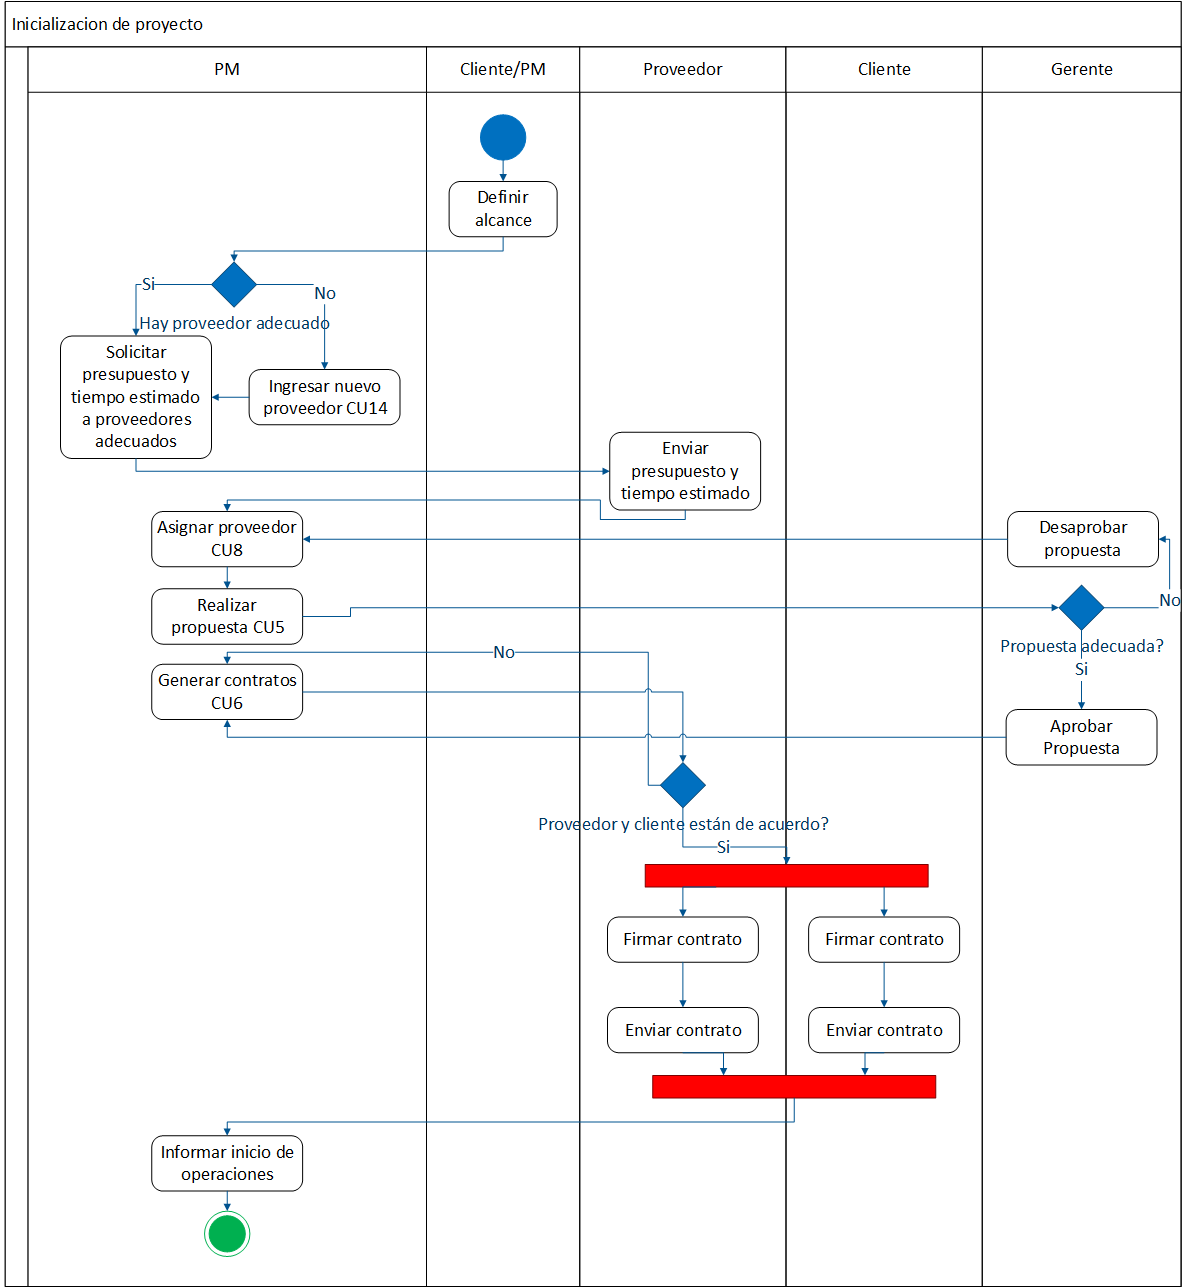
\includegraphics[width=1.15\textwidth]{images/InicProy.png}}
\makebox[\textwidth][c]{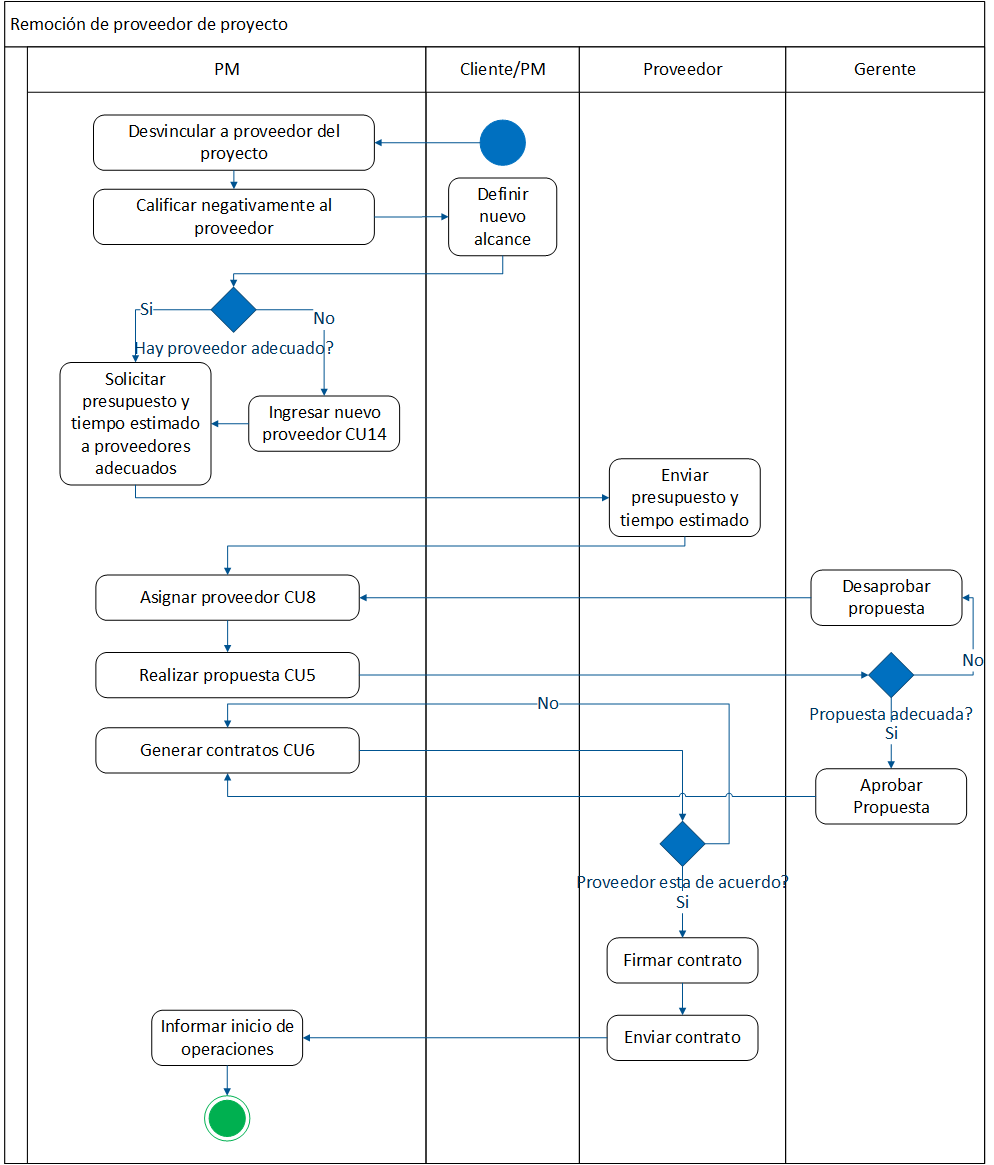
\includegraphics[width=1.15\textwidth]{images/CambProv.png}}
\makebox[\textwidth][c]{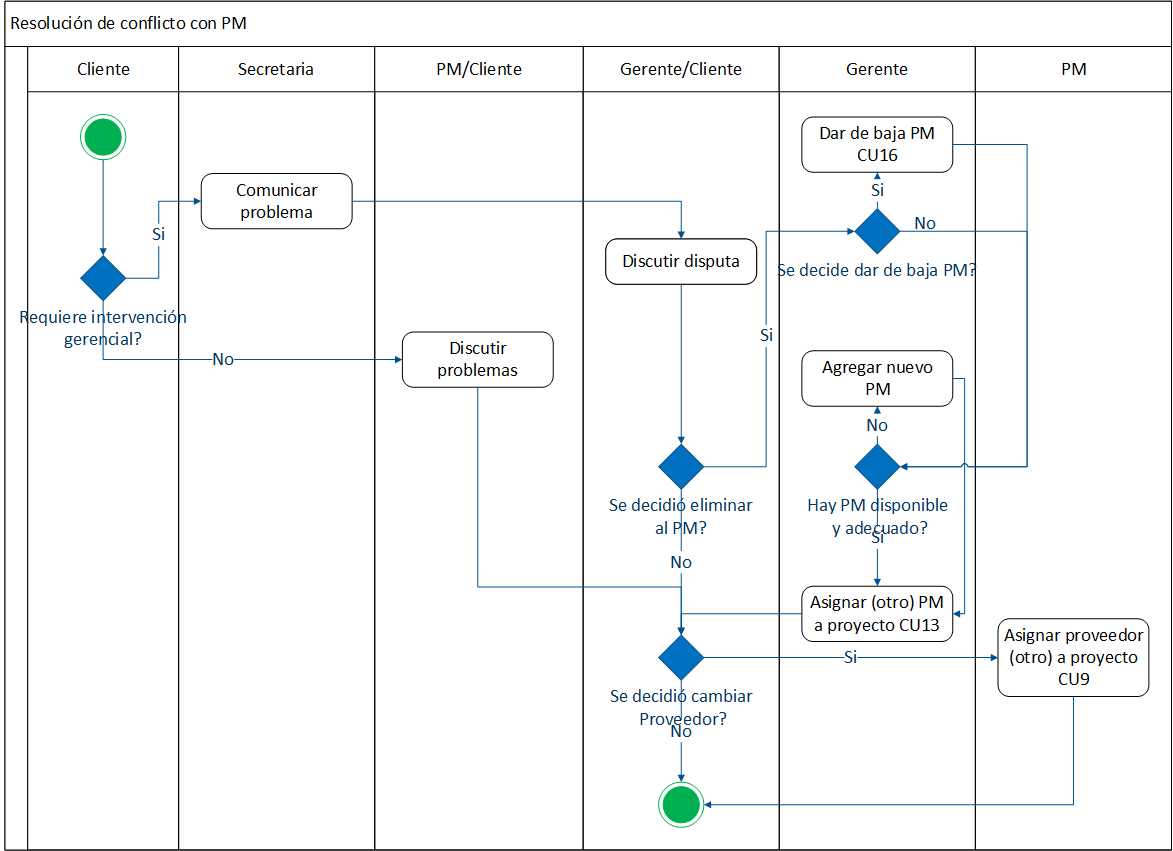
\includegraphics[width=1.15\textwidth]{images/ResConfl.png}}

\pagebreak

\section{Finite State Machine (FSM)}

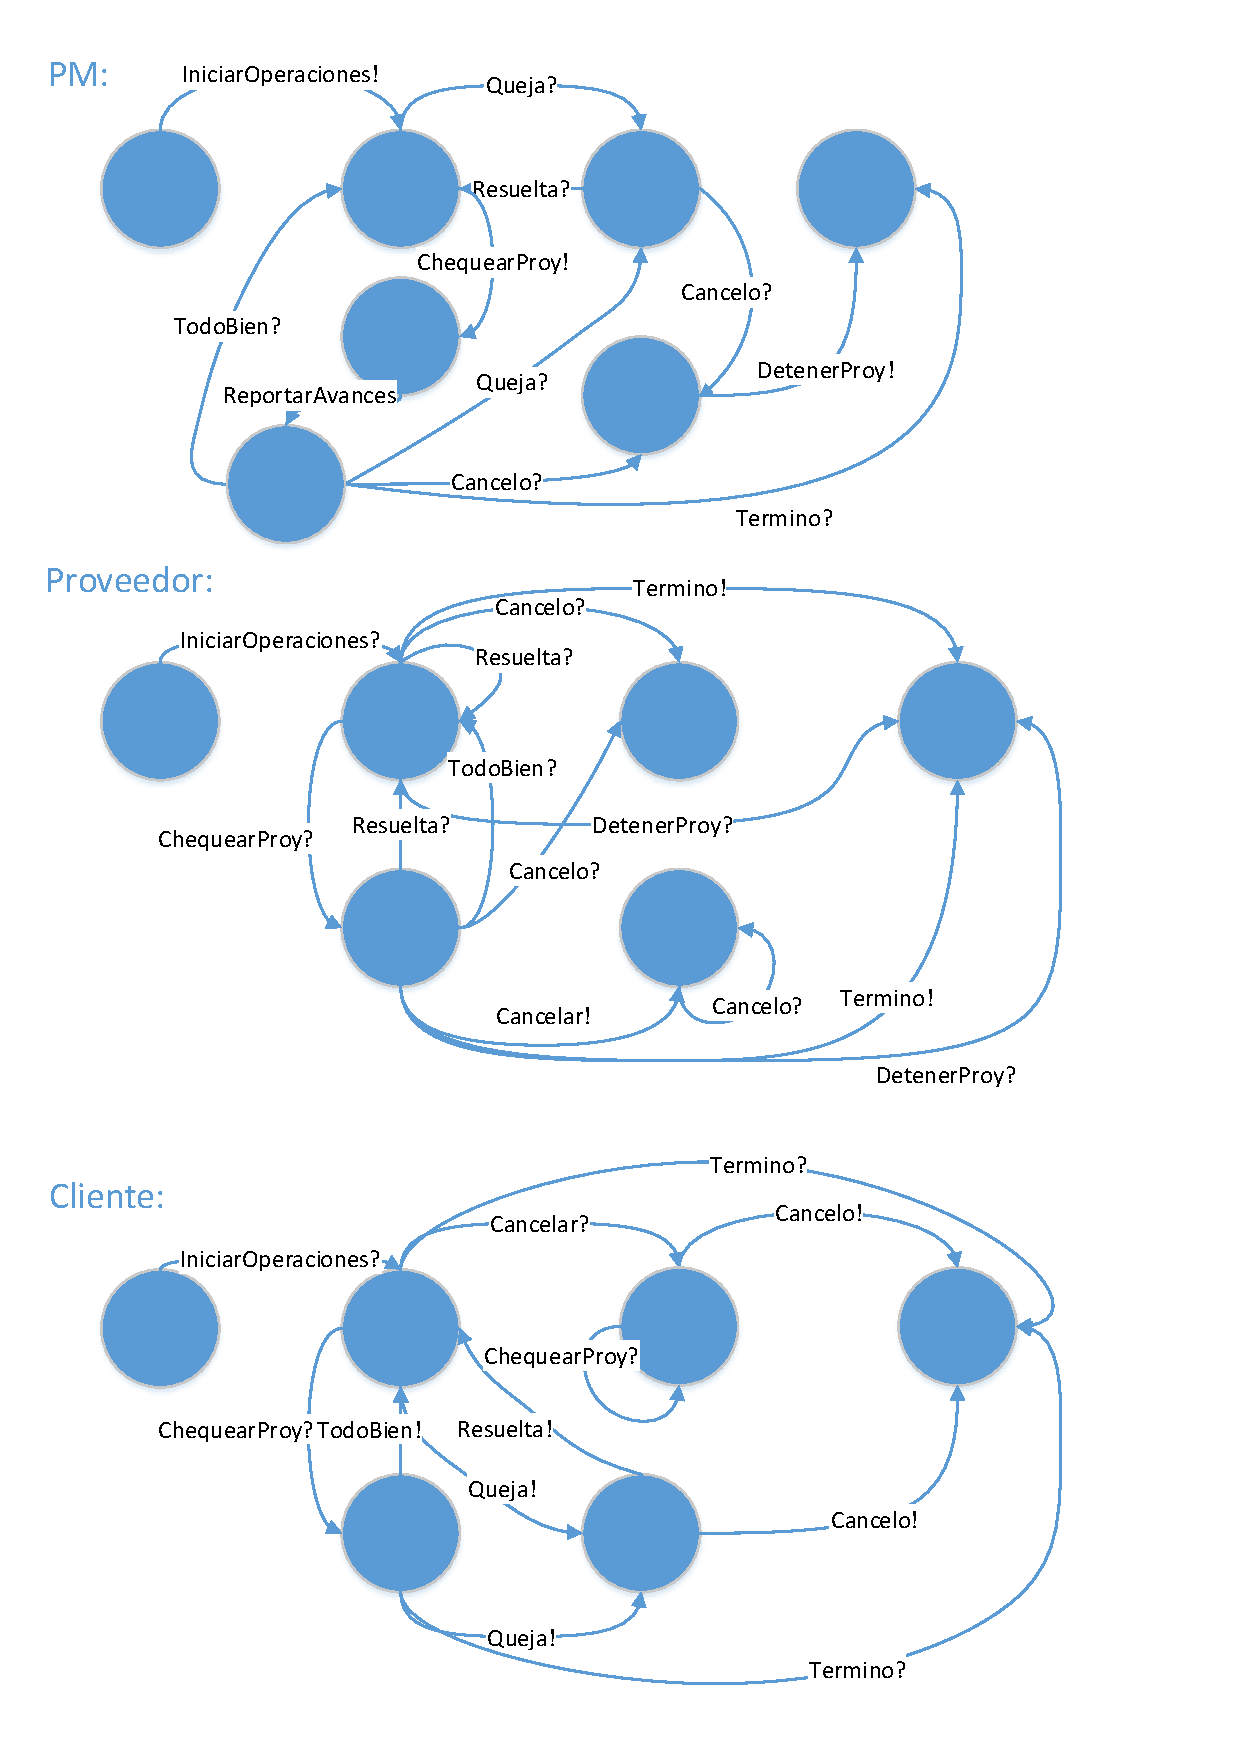
\includegraphics[width=\textwidth,height=\textheight,keepaspectratio,page=1]{images/state.pdf}
Algo para tener en cuenta es que 'Cancelo' o 'Cancelar' se refiere a la decisión desvinculación del proveedor del proyecto.

\section{Escenarios Hipotéticos}

%% \textbf{CORRECCION GERVA, LA DEJO COMO REFERENCIA, SACARLA DESPUES DEL INFORME!}

% De los escenarios
% En el primer escenario (6.1) se dice que “en caso de poseer acceso a internet inicia el pedido dirigiéndose a la página web de la empresa”. Pero ¿en el diagrama de contexto no se muestra que el cliente no interactúa nunca con nuestro sistema?

% Pasa algo parecido con el 6.2: el cliente tiene la posibilidad de completar una encuesta accediendo directamente al sistema.

% En el escenario 6.4 se presenta cómo es el PM el que hace llegar contrato a cliente y proveedor por fuera del sistema. ¿Está bueno eso? ¿No está bueno que la aceptación o rechazo de un presupuesto, de ambas partes, se pueda hacer interactuando con el sistema?

\subsection{Cliente solicita el servicio}

Un cliente necesita de los servicios de la empresa para poder completar su obra, en caso de poseer acceso a internet inicia el pedido dirigiéndose a la pagina web de la empresa. Mediante un formulario se le provee al cliente de un espacio para ingresar sus datos, su pedido y alguna dirección de correo para que desde la empresa sea posible comunicarse con el. Por otro lado, si el cliente no dispone de conexión a internet, este se comunica con la empresa vía telefónica con una secretaria, esta le solicita sus datos y en base a ellos carga en el sistema un formulario como el generado en el caso anterior, seguido de algún numero de teléfono por el cual pueda ser comunicado, y dejando además en claro que se trata de un cliente sin conexión a internet, por lo que dicho numero sera el canal principal de comunicación. El pedido es así entonces procesado e ingresado en el sistema, siendo agregado a la cola de proyectos.

\subsection{Cliente responde encuesta sobre los resultados de la obra}

Una vez que el PM correspondiente marca el proyecto como terminado, al cliente se le permite la opcion de realizar una encuesta final que refleje su opinión acerca de la calidad del servicio, esto es sumamente util ya que después estas opiniones se usan para calificar el PM.

\vspace{5px}

%De aquí pueden ocurrir dos alternativas para completar dicha encuesta: para aquellos casos en que se sepa que el cliente posee conexión a internet, se le envía un enlace el cual contiene un formulario donde puede expresar sus comentarios, y una vez que termina, el cliente procede a enviar el mismo mediante un botón en la pagina, el cual se encarga de cargar el formulario en el sistema. Por otro lado, para el caso de aquellos clientes que se sepa que no poseen una conexión a internet, el Centro de Atención al Cliente se encarga de hacerle una encuesta telefónica, de la cual se deriva un formulario que luego es cargado en el sistema.

\subsection{Secretaria actualiza la lista de proveedores}

La secretaria revisa la lista de proveedores actualmente contenida en el sistema que haya sido reportada por el mismo. En base a esta se encarga de solicitar a los correspondientes proveedores sus datos y comprobantes, en especial el del seguro al día. Luego dichos proveedores se encargaran de enviar toda la documentación pertinente.

\vspace{5px}

Dado el envió de nuevos datos y comprobantes de un proveedor, la secretaria se dedica a modificar la lista de proveedores, si se trata de un proveedor que ya figure allí se procede a actualizar sus datos, en caso contrario se registra al nuevo proveedor en la base de datos del sistema.

%\subsection{Cliente utiliza el servicio}
%Raimundo esta a cargo de la construcción de un edificio, la empresa encargada de las ventanas fallo. Envía un correo electrónico a DC construcciones, solicitando un presupuesto para instalar las ventanas en la obra y otorgando datos de contacto. El gerente selecciona un PM libre en el sistema y lo asigna al proyecto.
%El sistema encuentra a los mejores proveedores para este proyecto, el PM selecciona los necesarios y el sistema les envía una solicitud de presupuesto.

% (CHEQUEAR: DIAGRAMA DE CONTEXTO NO ESPECIFICA CONTACTO DIRECTO ENTRE PROVEEDORES Y SISTEMA)
%\vspace{5px}

%Los proveedores envían su presupuesto y el PM elije uno de los proveedores. Se verifica que el proveedor seleccionado este disponible y con el seguro al día.
%El PM ingresa el presupuesto del proveedor seleccionado al sistema y el Gerente lo aprueba.
%El PM negocia los términos del contrato con el cliente y el proveedor por separado, una vez que están claros carga la propuesta en el sistema. El gerente genera los contratos utilizando un tamplate del sistema. El PM hace llegar el contrato al cliente y el proveedor, y actualiza el estado del proyecto. El cliente y el proveedor firman los contratos y el PM lo notifica en el sistema. El proveedor comienza la obra y el PM actualiza el estado del proyecto. El proveedor finaliza la obra y el PM actualiza el estado del proyecto. El cliente esta satisfecho y completa la encuesta de satisfacción positivamente. 

\subsection{Proveedor no logra cumplir el contrato}
Estando el proyecto en marcha, el proveedor encargado de realizar los revoques cancela la operación. El PM notifica de esta situación al sistema, el PM encuentra un nuevo proveedor que puede completar el proyecto y lo ingresa al sistema junto con su presupuesto, el gerente aprueba el presupuesto. Se verifica que ese disponible y tenga el seguro al día. El PM negocia los términos con el nuevo proveedor, actualiza los datos en el sistema. El gerente esta de acuerdo y genera un contrato completo nuevo y lo ingresa al sistema. El PM lo hace llegar al proveedor y notifica al sistema. El proveedor firma y se reanuda la obra, el PM actualiza el proyecto.

\subsection{PM recibe muchas quejas del cliente}
Estando la construcción en marcha, el cliente no se siente conforme con el modo en el que se realizan los trabajos de parte de la empresa constructora y acude al PM para solucionarlo. El PM no le da ninguna solución porque esta ocupado con problemas personales y deja de atender los llamados del cliente. El cliente llama a la secretaria, deja su queja, y la secretaria lo carga en el sistema. El sistema notifica a los gerentes de esta situación. El gerente si lo ve pertinente comunica decisiones al PM actual, o asigna un nuevo PM al proyecto. En este ultimo caso es este nuevo PM el que esta a cargo de seguir este proyecto y asistir al cliente.

\subsection{Surgen cargos adicionales}
Comenzando la puesta en marcha de la construcción el proveedor indica que luego de colocar el sistema de calefacción también hay que colocar insulación en las paredes, esto no forma parte del contrato y ellos tampoco otorgan este servicio. El cliente notifica esta situación al PM requiriendo un proveedor adicional que le coloque la insulación. El PM carga un proyecto adicional vinculado al original. Se sigue el camino normal como un proyecto nuevo con la diferencia que no hay un nuevo contrato con el cliente, sino que este nuevo trabajo se agrega como clausula adicional al contrato del proyecto original.

\end{document}

